\documentclass[11pt,a4paper]{article}

\def\nyear {2025}
\def\nterm {Spring}
\def\nlecturer {Michah Sageev and notes by Nir Lazarovich}
\def\ncourse {Topology}

\makeatletter

% packages
\usepackage{amssymb,amsfonts,amsmath,calc,tikz,pgfplots,geometry,mathtools}
\usepackage{color}   % May be necessary if you want to color links
\usepackage[svgnames]{xcolor}
\usepackage[hidelinks]{hyperref}
\usepackage{forest}
\usepackage{commath} % ew
\usepackage{esvect} % \vv makes vectors
\usepackage{centernot} % for the comparison
\usepackage{esdiff}
\usepackage{esint}
\usepackage{amsthm}
\usepackage{fancyhdr}
\usepackage{bm}
\usepackage{witharrows}
\usepackage{bookmark}
\usepackage{tikz-cd}
\usepackage{quiver}
\usepackage{bbm}
\usepackage{textcomp}
\usepackage{float}
\usepackage{gensymb}
\usepackage{cleveref}
\usepackage{environ}
\usepackage{comment}
\usepackage{cancel}
\usepackage{xparse}

% Inevitable cs
\usepackage{listings}
\usepackage[]{algorithm2e}

% tikz libraries
\usetikzlibrary{positioning}
\usetikzlibrary{matrix}
\usetikzlibrary{arrows}
\usetikzlibrary{bending}
\usetikzlibrary{arrows.meta}
\usetikzlibrary{decorations.markings}
\usetikzlibrary{decorations.pathreplacing}
\usetikzlibrary{decorations.markings}
\usetikzlibrary{patterns}
\usetikzlibrary{backgrounds}

% Page style setup
\pagestyle{fancy}
\fancyhfoffset{0pt}
\renewcommand{\headwidth}{\textwidth}
\geometry{margin=1in}
\pgfplotsset{compat=1.18}
\setlength{\headheight}{14.6pt}
\addtolength{\topmargin}{-1.6pt}
\hypersetup{
    colorlinks=false,
    linktoc=section,
    linkcolor=black,
}

%% maketitle setup
\ifx \nauthor\undefined
  \def\nauthor{Yeheli Fomberg}
\else
\fi

\ifx \nemail\undefined
  \def\nemail{\href{mailto:yp@campus.technion.ac.il}
  {\texttt{<yp@campus.technion.ac.il>}}}
\else
\fi

\ifx \ncoursehead \undefined
  \def\ncoursehead{\ncourse}
\fi

\lhead{\emph{\nouppercase{\leftmark}}}
\ifx \nextra \undefined
  \rhead{
    \ifnum\thepage=1
    \else
      \ncoursehead
    \fi}
\else
  \rhead{
    \ifnum\thepage=1
    \else
      \ncoursehead \ (\nextra)
    \fi}
\fi

\def\notes{notes}
\def\problems{problems}

\ifx \ntype \undefined
  \def\ntype{notes}
\else
\fi

\ifx \ntype \notes
  \let\@real@maketitle\maketitle
  \renewcommand{\maketitle}{\@real@maketitle\begin{center}
  \begin{minipage}[c]{0.9\textwidth}\centering\footnotesize
  These notes are not endorsed by the lecturers.
  I have revised them outside lectures to incorporate supplementary
  explanations, clarifications, and material for fun.
  While I have strived for accuracy, any errors or misinterpretations 
  are most likely mine.
  \end{minipage}\end{center}}
\else
  \ifx \ntype \problems
    \let\@real@maketitle\maketitle
    \renewcommand{\maketitle}{\@real@maketitle\begin{center}
    \begin{minipage}[c]{0.9\textwidth}\centering\footnotesize
    These problems are mostly based on the problem sets I was given
    when taking the course.
    
    While I have strived for accuracy and completeness,
    some of the problems would not have been here without the help of
    friends.
    \end{minipage}\end{center}}
  \else
  \fi
\fi


% theorem environments
\theoremstyle{definition}
\newtheorem{definition}{Definition}[section]
\newtheorem{remark}{Remark}[section]
\newtheorem{example}{Example}[section]
\newtheorem{exercise}{Exercise}[section]
\newtheorem{paradox}{Paradox}[section]
\newtheorem{entry}{Entry}[section]
\newtheorem*{solution}{Solution}
\newtheorem*{question}{Question}
\newtheorem*{answer}{Answer}
\newtheorem*{problem}{Problem}
\theoremstyle{plain}
\newtheorem{theorem}{Theorem}[section]
\newtheorem{proposition}[theorem]{Proposition}
\newtheorem{lemma}[theorem]{Lemma}
\newtheorem{corollary}[theorem]{Corollary}
\newenvironment{proofof}[1]{%
    \renewcommand{\proofname}{Proof of #1}%
    \begin{proof}
}{%
    \end{proof}
}
% tikz customization
\pgfarrowsdeclarecombine{twolatex'}{twolatex'}{latex'}{latex'}{latex'}{latex'}
\tikzset{->/.style = {decoration={markings,
                                  mark=at position 0.999
                                  with {\arrow[scale=2]{latex'}}},
                      postaction={decorate}}}
\tikzset{<-/.style = {decoration={markings,
                                  mark=at position 0.001 with {\arrowreversed[scale=2]{latex'}}},
                      postaction={decorate}}}
\tikzset{-->/.style = {decoration={markings,
                                  mark=at position 0.999
                                  with {\arrow[scale=2]{latex'[sep=0pt -2.5]}}},
                      postaction={decorate}}}
\tikzset{<--/.style = {decoration={markings,
                                  mark=at position 0.001
                                  with {\arrowreversed[scale=2]{latex'[sep=0pt -2.5]}}},
                      postaction={decorate}}}
\tikzset{<->/.style = {decoration={markings,
                                  mark=at position 0.001 with {\arrowreversed[scale=2]{latex'}},
                                  mark=at position 0.999 with {\arrow[scale=2]{latex'}},},
                      postaction={decorate}}}
\tikzset{->-/.style = {decoration={markings,
    mark=at position 0.50+0.225/#1 with {\arrow[scale=2]{latex'}}},
                      postaction={decorate}}}
\tikzset{-<-/.style = {decoration={markings,
                                   mark=at position 0.50-0.225/#1 with {\arrowreversed[scale=2]{latex'}}},
                       postaction={decorate}}}
\tikzset{->>/.style = {decoration={markings,
                                  mark=at position 1 with {\arrow[scale=2]{latex'}}},
                      postaction={decorate}}}
\tikzset{<<-/.style = {decoration={markings,
                                  mark=at position 0 with {\arrowreversed[scale=2]{twolatex'}}},
                      postaction={decorate}}}
\tikzset{<<->>/.style = {decoration={markings,
                                   mark=at position 0 with {\arrowreversed[scale=2]{twolatex'}},
                                   mark=at position 1 with {\arrow[scale=2]{twolatex'}}},
                       postaction={decorate}}}
\tikzset{->>-/.style = {decoration={markings,
                                   mark=at position 0.50+0.450/#1 with {\arrow[scale=2]{twolatex'}}},
                       postaction={decorate}}}
\tikzset{-<<-/.style = {decoration={markings,
                                   mark=at position 0.50-0.450/#1 with {\arrowreversed[scale=2]{twolatex'}}},
                       postaction={decorate}}}

\pgfarrowsdeclare{biggertip}{biggertip}{%
  \setlength{\arrowsize}{1pt}
  \addtolength{\arrowsize}{.1\pgflinewidth}
  \pgfarrowsrightextend{0}
  \pgfarrowsleftextend{-5\arrowsize}
}{%
  \setlength{\arrowsize}{1pt}
  \addtolength{\arrowsize}{.1\pgflinewidth}
  \pgfpathmoveto{\pgfpoint{-5\arrowsize}{4\arrowsize}}
  \pgfpathlineto{\pgfpointorigin}
  \pgfpathlineto{\pgfpoint{-5\arrowsize}{-4\arrowsize}}
  \pgfusepathqstroke
}
\tikzset{
	EdgeStyle/.style = {>=biggertip}
}

\tikzset{circ/.style = {fill, circle, inner sep = 0, minimum size = 3}}
\tikzset{scirc/.style = {fill, circle, inner sep = 0, minimum size = 1.5}}
\tikzset{mstate/.style={circle, draw, black, text=black, minimum width=0.7cm}}

\tikzset{eqpic/.style={baseline={([yshift=-.5ex]current bounding box.center)}}}

\definecolor{mblue}{rgb}{0.2, 0.3, 0.8}
\definecolor{morange}{rgb}{1, 0.5, 0}
\definecolor{mgreen}{rgb}{0, 0.4, 0.2}
\definecolor{mred}{rgb}{0.5, 0, 0}

% topology
\DeclareMathOperator{\dfr}{dfr} % deformation retract
\newcommand{\Cells}{\text{Cells}}
\newcommand{\RP}{\mathbb{RP}}
\newcommand{\CP}{\mathbb{CP}}

% order theory
\newcommand{\join}{\vee}
\newcommand{\meet}{\wedge}

% algebraic geometry
\DeclareMathOperator{\Rad}{Rad} % Radical of modules
\DeclareMathOperator{\Spec}{Spec}
% \renewcommand{\div}{\mathrm{div}} % divisors
\DeclareMathOperator{\Mer}{Mer} % Meromorphic functions
\DeclareMathOperator{\Exc}{Exc} % Exceptional divisor
\DeclareMathOperator{\Td}{Td} % Todd classes

% algebra

\DeclareMathOperator{\trdeg}{tr.deg.}
\DeclareMathOperator{\odd}{odd}
\DeclareMathOperator{\even}{even}
\DeclareMathOperator{\lcm}{lcm}
\DeclareMathOperator{\ord}{ord}
\DeclareMathOperator{\codim}{codim}
\DeclareMathOperator{\Ann}{Ann}
\DeclareMathOperator{\Ext}{Ext}
\DeclareMathOperator{\Sym}{Sym}
\DeclareMathOperator{\Out}{Out}
\DeclareMathOperator{\Aut}{Aut}
\DeclareMathOperator{\End}{End}
\DeclareMathOperator{\Inn}{Inn}
\DeclareMathOperator{\Mat}{Mat}
\DeclareMathOperator{\Fix}{Fix}
\DeclareMathOperator{\std}{std}
\DeclareMathOperator{\sgn}{sgn}
\DeclareMathOperator{\adj}{adj}
\DeclareMathOperator{\id}{id}
\DeclareMathOperator{\op}{op}
\DeclareMathOperator{\tr}{tr}
\DeclareMathOperator{\diag}{diag}
\DeclareMathOperator{\rank}{rank}
\DeclareMathOperator{\rk}{rk}
\DeclareMathOperator{\coker}{coker}
\DeclareMathOperator{\Mult}{Mult} % multiplier algebra
\DeclareMathOperator{\Frac}{Frac} % fraction field
\DeclareMathOperator{\Rat}{Rat}
\DeclareMathOperator{\Gal}{Gal}
\newcommand{\ioplus}{\overset{\text{int}}{\oplus}} % interior direct sum
\newcommand{\GG}{\mathcal G} % Galois correspondence
\newcommand{\FF}{\mathcal F} % Galois correspondence
\newcommand{\cupp}{\smile} % cup product
\newcommand{\capp}{\frown} % cap product
\newcommand{\actson}{\curvearrowright}
\newcommand{\bra}{\left\langle}
\newcommand{\ket}{\right\rangle}
\newcommand{\idealin}{\triangleleft\,}
\newcommand{\normalin}{\triangleleft\,}
\newcommand{\ip}[2]{\left\langle #1, #2 \right\rangle}
\newcommand{\bigslant}[2]
{{\raisebox{.2em}{$#1$}\left/\raisebox{-.2em}{$#2$}\right.}}
\newcommand{\properideal}{%
  \mathrel{\ooalign{$\lneq$\cr\raise.22ex\hbox{$\lhd$}\cr}}}

% categories
\newcommand{\cat}[1]{\mathbf{#1}}
\newcommand{\Ch}{\cat{Ch}} % Chain complexes   
\newcommand{\Set}{\cat{Set}}
\newcommand{\Grp}{\cat{Grp}}
\newcommand{\Ab}{\cat{Ab}}
\newcommand{\Ring}{\cat{Ring}}
\newcommand{\CRing}{\cat{CRing}}
\newcommand{\Top}{\cat{Top}}
\newcommand{\Vect}{\cat{Vect}}
\newcommand{\cmod}{\cat{mod}}

%% matrix groups
\newcommand{\GL}{\mathrm{GL}}
\newcommand{\Or}{\mathrm{O}}
\newcommand{\PGL}{\mathrm{PGL}}
\newcommand{\PSL}{\mathrm{PSL}}
\newcommand{\PSO}{\mathrm{PSO}}
\newcommand{\PSU}{\mathrm{PSU}}
\newcommand{\SL}{\mathrm{SL}}
\newcommand{\msl}{\mathrm{sl}}
\newcommand{\SO}{\mathrm{SO}}
\newcommand{\Spin}{\mathrm{Spin}}
\newcommand{\Sp}{\mathrm{Sp}}
\newcommand{\SU}{\mathrm{SU}}
\newcommand{\U}{\mathrm{U}}
\let\char\relax
\newcommand{\char}{\text{char}}

% analysis
\renewcommand{\Re}{\mathrm{Re}}
\renewcommand{\Im}{\mathrm{Im}}
\NewDocumentCommand{\dx}{o}{
  \IfNoValueTF{#1}
    {\dif x}                  % if no optional argument
    {\dif^{#1} \!x}         % if optional argument
}
\NewDocumentCommand{\dy}{o}{
  \IfNoValueTF{#1}
    {\dif y}                  % if no optional argument
    {\dif^{#1} \!y}         % if optional argument
}
\newcommand{\dt}{\dif t}
\newcommand{\du}{\dif u}
\newcommand{\dv}{\dif v}
\newcommand{\dz}{\dif z}
\newcommand{\ds}{\dif s}
\newcommand{\dw}{\dif w}
\newcommand{\dr}{\dif r}
\newcommand{\dm}{\dif m}
\newcommand{\df}{\dif f}
\newcommand{\dV}{\dif V}
\newcommand{\dS}{\dif S}
\newcommand{\dA}{\dif \mathrm{A}}
\newcommand{\dmu}{\dif \mu}
\newcommand{\dnu}{\dif \nu}
\newcommand{\dtheta}{\dif \theta}
\newcommand{\domega}{\dif \omega}
\newcommand{\dsigma}{\dif \sigma}
\newcommand{\dtau}{\dif \tau}
\newcommand{\dvarphi}{\dif \varphi}
\renewcommand{\dif}{\mathrm{d}}
\renewcommand{\Dif}{\mathrm{D}}
\renewcommand{\triangle}{\Delta}
\newcommand{\ptriangle}{\partial \triangle}
\DeclareMathOperator{\im}{im}
\DeclareMathOperator{\cis}{cis}
\DeclareMathOperator{\rot}{rot}
\DeclareMathOperator{\vspan}{span}
\DeclareMathOperator{\grad}{grad}
\DeclareMathOperator{\curl}{curl}
\DeclareMathOperator{\esssup}{esssup}
\newcommand{\hodge}{{\mathnormal{\star}}}
\DeclareMathOperator{\range}{range}
\DeclareMathOperator{\Hom}{Hom}
\DeclareMathOperator{\Int}{Int}
\DeclareMathOperator{\Conv}{Conv} % convex hull
\newcommand{\ind}{\mathbbm{1}}
\DeclareMathOperator{\Res}{Res}
\DeclareMathOperator{\graph}{graph}
\DeclareMathOperator{\diam}{diam}
\DeclareMathOperator{\supp}{supp}
\DeclareMathOperator{\Vol}{Vol} % Volume
\DeclareMathOperator{\Area}{Area} % Area
\DeclareMathOperator{\area}{area}
\DeclareMathOperator{\Ind}{Ind} % Index
\newcommand{\length}{\mathrm{length}}

% logic
\DeclareMathOperator{\MOD}{MOD}
\DeclareMathOperator{\Theory}{Theory}
\newcommand{\notimplies}{%
  \mathrel{{\ooalign{\hidewidth$\not\phantom{=}$\hidewidth\cr$\implies$}}}}

% nice
\newcommand{\half}{\frac{1}{2}}
\newcommand{\pair}{\del}
\newcommand{\taking}[1]{\xrightarrow{#1}}
\newcommand{\otaking}[1]{\xleftarrow{#1}}
\newcommand{\inv}{^{-1}}
\newcommand{\ot}{\leftarrow}
\newcommand{\ninfty}{-\infty}
\newcommand{\pinfty}{+\infty}
\newcommand{\floor}[1]{\left\lfloor #1 \right\rfloor}
\newcommand{\ceil}[1]{\left\lceil #1 \right\rceil}
\newcommand{\viff}{\Big\Updownarrow} % vertical iff
\newcommand{\bmid}{\,\middle\vert\,} % big mid

% probability
\newcommand{\Prob}{\mathbf{P}}
\renewcommand{\vec}[1]{\boldsymbol{\mathbf{#1}}}
\DeclareMathOperator{\Bin}{Bin}
\DeclareMathOperator{\Geo}{Geo}
\DeclareMathOperator{\Poi}{Poi}
\DeclareMathOperator{\Exp}{Exp}
\DeclareMathOperator{\Var}{Var} % Variance
\DeclareMathOperator{\Cov}{Cov}

% special letters
\newcommand{\N}{\mathbb{N}}
\newcommand{\Z}{\mathbb{Z}}
\newcommand{\Q}{\mathbb{Q}}
\newcommand{\R}{\mathbb{R}}
\newcommand{\C}{\mathbb{C}}
\newcommand{\F}{\mathbb{F}}
\newcommand{\E}{\mathbf{E}}
\newcommand{\D}{\mathbb{D}}
\renewcommand{\H}{\mathbb{H}}
\newcommand{\ps}{\mathcal{P}}
\newcommand{\M}{\mathcal{M}}
\renewcommand{\L}{\mathcal{L}}
\renewcommand{\O}{\mathcal{O}}
\renewcommand{\U}{\mathcal{U}}
\newcommand{\Omicron}{O}
\newcommand{\powerset}{\mathcal{P}}

% text
\newcommand{\st}{\text{ s.t. }}
\newcommand{\tand}{\quad \text{and} \quad}
\newcommand{\tor}{\quad \text{or} \quad}
\newcommand{\stand}{\text{ and }}
\newcommand{\stor}{\text{ or }}
\renewcommand{\tt}[1]{\textnormal{\textbf{(#1).}}} %tt=theorem title GET RID OF

% title format
\title{\textbf{\ncourse}}

\ifx \ntype \notes
  \author{Notes taken by \nauthor\, \nemail \\ Based on lectures by \nlecturer}
  \date{\nterm\ \nyear}
\else
  \ifx \ntype \problems
    \author{These problems were solved by \nauthor \\ \nemail}
  \else
  \fi
\fi

\makeatother


\begin{document}
\maketitle

% Insert cool image here

\newpage
\tableofcontents
\newpage

\setcounter{section}{-1}

\section{Introduction}

Before getting into the main part of the course, we can first look
at topology from the viewpoint it was considered hundreds of years ago.

\begin{definition}[Geodesic triangle]
  A geodesic triangle is the area enscribed inside $3$ points
  on a sphere.
\end{definition}

\begin{theorem}[Girard's theorem]
  \label{thm:girard}
  Let $T$ be a geodesic triangle.
  Denote its angles $\theta_1$, $\theta_2$, $\theta_3$.
  Then we have $\theta_1 + \theta_2 + \theta_3 > 180^{\circ}$ and
  \[
    \mathrm{Area}(T) = \theta_1 + \theta_2 + \theta_3 - \pi.
  \]
\end{theorem}
\begin{proof}
  Geometric.
\end{proof}

\begin{theorem}[Euler's theorem]
  \label{thm:euler}
  Let $P$ be a convex polyhydron.
  Denote $E$ the number of edges in $P$, $V$ the number of vertices in $P$,
  and $F$ the number of faces of $P$.
  Then
  \[
    V - E + F = 2.
  \]
\end{theorem}
\begin{proof}
  Begin by ensphering the polyhydron in the unit sphere.
  Put a flashlight inside the polyhydron such that the faces of $P$
  cast shadows of geodesic polygons on the sphere.
  Then we triangulate all the geodesic polygons.
  We have
  \[
    \boxed{2 E = 3 F}
  \]
  Denote the trianlges $\sigma_1,\dots,\sigma_F$.
  From \Cref{thm:girard} we have that
  \[
    \sum_{i=1}^{F} \frac{\theta_1^i + \theta_2^i + \theta_3^i}{V} - \pi =
    4 \pi.
  \]
  From this we get
  \[
    2 \pi V - \pi F = 4 \pi \implies
    \boxed{2 V - F = 4}
  \]
  From these equations we can deduce the desired relation
  \[
    \boxed{V - E + F = 2}
  \]
  which completes the proof.
\end{proof}

\begin{remark}
  We saw in \Cref{thm:euler} that the value of $V - E + F$ is constant
  for convex polygons, and that it is always equal to $2$.
  However, if we consider a box with a hole in it
  \begin{center}
    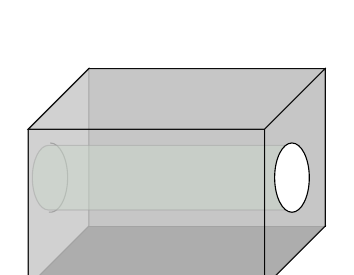
\begin{tikzpicture}
      \newcommand{\Depth}{3}
      \newcommand{\Height}{2}
      \newcommand{\Width}{2}
      \coordinate (O) at (0,0,0);
      \coordinate (A) at (0,\Width,0);
      \coordinate (B) at (0,\Width,\Height);
      \coordinate (C) at (0,0,\Height);
      \coordinate (D) at (\Depth,0,0);
      \coordinate (E) at (\Depth,\Width,0);
      \coordinate (F) at (\Depth,\Width,\Height);
      \coordinate (G) at (\Depth,0,\Height);
      \draw[fill=black!80] (O) -- (C) -- (G) -- (D) -- cycle;% Bottom Face
      \draw[fill=black!30] (O) -- (A) -- (E) -- (D) -- cycle;% Back Face
      \draw[fill=black!10] (O) -- (A) -- (B) -- (C) -- cycle;% Left Face
      \draw[scale=1.1] (-0.445,0.96)
        arc[end angle=-95, start angle=90, x radius=0.2cm, y radius=0.4cm];
      \node[cylinder, draw, shape aspect=.5,  
            cylinder uses custom fill, cylinder end fill=white!50, 
            minimum height=1cm,
            cylinder body fill=green!25, opacity=0.5, 
          scale=3.5] at (1.2,1,1) {};
      \draw[fill=black!20,opacity=0.8] (D) -- (E) -- (F) -- (G) -- cycle;% Right Face
      \draw[fill=black!20,opacity=0.8] (C) -- (B) -- (F) -- (G) -- cycle;% Front Face
      \draw[fill=black!20,opacity=0.8] (A) -- (B) -- (F) -- (E) -- cycle;% Top Face
      \draw[scale=1.1,fill=white] (2.345,0.56) ellipse (0.2cm and 0.4cm);
    \end{tikzpicture}
  \end{center}
  and treat the ellipses as empty rectangles connected by $4$ edges each
  from their own vertices to the vertices of the face that contains the hole
  they represent, we get that
  \[
    F - E + V = 16 - 32 + 16 = 0
  \]
  which tells us that there is more to Euler's theorem than we may think.
\end{remark}

\newpage

\section{Quotient spaces and complexes}

\subsection{Quotient spaces}

\begin{definition}[Quotient space]
  Let $(X, \tau)$ be a topological space, and let $\sim$ be an equivalence
  relation on $X$.
  Recall that the equivalence class of $x$ is given by:
  \[
    [x] := \set{y \in X \mid y \sim x}.
  \]
  We then define the quotient space by $X/{\sim} := \set{[x] \mid x \in X}$.
  We also define the projection map $\pi \colon X \to {X}/{\sim}$ by
  $\pi(x) = [x]$.
\end{definition}

\begin{definition}[Quotient topology]
  We define the quotient topology $\tau_{\sim}$ on ${X} / {\sim}$
  by $U \in \tau_{\sim}$ if and only if $\pi^{-1}(U) \in \tau$.
  In other words, the quotient topology is the final topology induced by $\pi$.
\end{definition}

\begin{proposition}[Universal property of quotient spaces]
  Let $X$, $Y$ be topological spaces, let $\sim$ be an equivalence relation
  on $X$, and let $f \colon X \to Y$ be a function such that for every 
  $x \sim x' \in X$ we have $f(x) = f(x')$.
  Then there exists a unique map $g \colon {X}/{\sim} \to Y$ such that
  $g \circ \pi = f$ where $\pi$ is the quotient projection.
  Moreover, $g$ is continuous if and only if $f$ is continuous.
  This property can be represented by the following
  commutative diagram:
  \[\begin{tikzcd}[ampersand replacement=\&,cramped]
    X \\
    \\
    {X/{\sim}} \&\& Y
    \arrow["\pi"', from=1-1, to=3-1]
    \arrow["f", from=1-1, to=3-3]
    \arrow["{g}"', dashed, from=3-1, to=3-3]
  \end{tikzcd}\]
\end{proposition}
\begin{proof}
  The first part of the proof is clear, so we will focus on the equivalence
  of continuity between $f$ and $g$.
  It is clear that $\pi$ is continuous so when $g$ is continuous
  we also have that $f = g \circ \pi$ is continuous.

  Next suppose $f$ is continuous.
  We need to show that for any open subset $V \subseteq Y$
  we have that $U := g^{-1}(V)$ is an open subset in $X/{\sim}$.
  Note that by commutativity of the diagram:
  \[
    \pi^{-1}(U) =
    \pi^{-1}(g^{-1}(V)) =
    f^{-1}(V),
  \]
  and since $V$ is open and $f$ is continuous we get that
  $\pi^{-1}(U) = f^{-1}(V)$ is open in $X$.
  By definition of the quotient topology,
  we get that $U$ is open in $X/{\sim}$, which completes the proof.
\end{proof}

\begin{example}[The unit sphere]
  Let $X = [0,1]$ with the topology induced by the standard topology on $\R$.
  Let $\sim$ be the equivalence relation generated by $0 \sim 1$.
  Then,
  \[
    {X}/{\sim} \cong S^1 =
    \{z \in \C^2 \mid |z| = 1\}.
  \]
  We define $f \colon X \to S^1$ by $f(t) = e^{2 \pi i t}$.
  Since $f$ is continuous and $f(0) = f(1)$, from the universal property
  of quotient spaces, there exists a continuous function 
  $g \colon {X}/{\sim} \to S^1$ defined by $g\del{[x]} = f(x)$.
  It is clear that $f$ is one to one and onto.
  In order to show that it is a homeomorphism we can use the following lemma.
  \begin{lemma}
    \label{lem:conditions-to-homeomorphism}
    Let $X$, $Y$ be topological spaces.
    Suppose that $X$ is compact, and $Y$ is Hausdorff.
    Then every continuous function from $X$ to $Y$ is a closed map.
    In particular, if $f$ is a continuous bijection, it is a homeomorphism.
  \end{lemma}
  \begin{proof}
    Let $C$ be a closed set in $X$.
    Since $X$ is compact $C$ is compact.
    Since $f$ is continuous $f(C)$ is compact in the Hausdorff space $Y$
    and thus closed which completes the proof.
  \end{proof}
  \begin{remark}
    In order to prove a compact subset $D$ of a Hausdorff space $Y$ is closed,
    we will show that $Y \setminus D$ is open.
    Let $x \in Y \setminus D$ be given.
    Since $Y$ is Hausdorff, for every $y \in D$ there exist neighbourhoods
    $U_y$ and $V_y$ such that $x \in U_y$ and $y \in V_y$ and
    $U_y \cap V_y = \emptyset$.
    Clearly $\{V_y\}_{y \in D}$ is an open cover of $D$, so it has
    a finite subcover $\{V_y\}_{y \in I}$ for some finite set $I \subset D$.
    We therefore have that the set $U = \bigcap_{y \in I} U_y$ is an open
    neighbourhood of $x$, and $U \cap D = \emptyset$.
    This completes the proof.
  \end{remark}
\end{example}

\begin{exercise}
  Show that
  $X = {\C \setminus \set{0}}/{x \sim \lambda x} \quad
  \forall 0 \neq \lambda \in \R$
  is homeomorphic to the unit sphere $S^1$.
\end{exercise}
\begin{solution}
  First define the function $f \colon \C \setminus \set{0} \to S^1$ by
  \[
    f(z) = \frac{z}{|z|}.
  \]
  The function $f$ is continuous and satisfies $f(x) = f(\lambda x)$ for all
  $0 \neq \lambda \in \R$.
  Thus, from the universal property of quotient spaces there exists
  a continuous function $g \colon X \to S^1$.
  We will show that $f$ is one to one and onto.
  We have that $X = \pi(S^1)$ because every element in $\C \setminus \set{0}$
  is equivalent to some element in $S^1$, and since $\pi$ is continuous
  and $S^1$ is compact, it follows that $X$ is also compact.
  It is clear that $S^1$ is Hausdorff, and thus by
  \Cref{lem:conditions-to-homeomorphism}
  we have that $g$ is a homeomorphism between $X$ and $S^1$.
\end{solution}

\begin{remark}
  From now on we denote
  \begin{align*}
    &\text{The $n$-disc:} &&D^n := \{x \in \R^n \colon \norm{x} \le 1\}; \\
    &\text{The $n$-sphere:} &&S^n := \partial D^{n+1} = \{x \in \R^{n+1} \colon \norm{x} = 1\}; \\
    &\text{The $n$-torus:} &&T^n := (S^1)^n.
  \end{align*}
\end{remark}

\begin{remark}
  The $1$-torus is defined to be the $1$-sphere.
  This is why in some areas of math (especially analysis),
  people sometimes use the notation $T$ for the unit circle.
\end{remark}

\begin{remark}
  We notice that $D^0 = \set{0}$ and $\partial D^0 = \emptyset$ and
  $S^0 = \set{-1, 1}$.
\end{remark}

\begin{example}
  We have that $D^n / S^{n-1} \cong S^n$.
  The equivalence relation here is $x \sim y$ if and only if $x,y \in S^{n-1}$.
  Intuitively, we glue $S^{n-1}$ to a single point in space, resulting
  in $S^n$.
\end{example}
\begin{example}
  We have that $\R / \Z \cong S^1$ where $x \sim x + k$ for all
  $x \in \R$, $k \in \Z$.
\end{example}
\begin{example}
  For all $x \in \R^n \setminus \set{0}$ and $\lambda \in (0,\infty)$ we
  have:
  \[
    S^{n-1} \cong {\R^n \setminus \set{0}}/{x \sim \lambda x}.
  \]
\end{example}

\subsection{Pastings}

The following lemma will allow us to discuss more pastings of spaces.

\begin{lemma}
  Let $X$ be a topological space,
  let $\sim$ an equivalence relation on $X$,
  let $\pi$ the quotient projection,
  and let $f \colon X \to Y$ be a continuous function such that:
  \begin{enumerate}
    \item[(1)] $f$ is constant on the fibers of $\pi$.
    \item[(2)] $f'$ is one to one and onto.
    \item[(3)] $f$ is closed, open, or (${X}/{\sim}$ is compact and
      $Y$ is Hausdorff).
  \end{enumerate}
  Then $f'$ is a homeomorphism.
\end{lemma}

\begin{example}
  Let $X = [0,1] \cup [2,3]$ and $\sim := 1 \sim 2$.
  Then ${X}/{\sim} = [0,2]$.
  We can see this by defining the function $f \colon X \to [0,2]$ as such
  \[
    x \mapsto
    \begin{cases}
      x, & 0 \le x \le 1 \\
      x - 1, & 2 \le x \le 3
    \end{cases}.
  \]
\end{example}

\begin{example}
  Define
  \begin{align*}
    \R_n^+ &= \set{(x_1,\dots,x_n) \mid x_i \geq 0 } \\
    \R_n^- &= \set{(x_1,\dots,x_n) \mid x_i \le 0 }
  \end{align*}
  Define $X = \R_n^+ \cup \R_n^+$ (note that we treat this as a disjoint union).
  We define the equivalence relation 
  $(x_1^+,\dots,x_{n-1}^+, 0) \sim (x_1^-,\dots,x_{n-1}^-,0)$
  and then we have $\R^n \cong {X}/{\sim}$.
\end{example}

\begin{example}
  Let $X = I \times I$ where $I = [0,1]$.
  We define the equivalence relation as such $(s,0) \sim (s,1)$ for all
  $0 \le s \le 1$.
  Then ${X}/{\sim}$ is homeomorphic to a cylinder.
  We can see this by defining the function
  \[
    \fullfunction{f}{I \times I}{S \times I}
    {(s,t)}{(\cos 2 \pi t, \sin 2 \pi t, s)}
  \]
\end{example}

\begin{example}
  Let $X = I \times I$.
  Define the equivalence relation $(s, 0) \sim (1 - s, 1)$.
  The space ${X}/{\sim}$ is homeomorphic to a Mobius strip.
\end{example}

\begin{example}
  Let $X = I \times I$.
  Define the equivalence relation $(s, 0) \sim (s, 1)$ and 
  $(0, t) \sim (1, t)$.
  The space ${X}/{\sim}$ is homeomorphic to a torus (specifically
  $T^2$).
\end{example}

\subsection{CW complexes}

\subsubsection{Disjoint union}

\begin{definition}[Disjoint union topology]
  Let $\set{X_{\alpha}}_{\alpha}$ be a collection of topological spaces.
  We define the disjoint union topology in the following manner.
  We say that $U \subset \bigsqcup_{\alpha} X_{\alpha}$ is open if and only
  if $U \cap X_{\alpha}$ is open in $X_{\alpha}$ for any $X_{\alpha}$.
\end{definition}

\begin{example}
  If every $X_{\alpha}$ is endowed with the discrete topology,
  then any disjoint union of points is an open set 
\end{example}

\begin{example}
  We have that $D^1 \sqcup D^1 \cong [0,1] \cup [2,3]$ with the standard
  topology.
\end{example}

\begin{proposition}[Universal property of disjoint union]
  Let $\set{X_{\alpha}}_{\alpha}, Y$ be topological spaces,
  let $f_{\alpha} \colon X_{\alpha} \to Y$ be a collection of continuous
  functions.
  Then there exists a unique continuous function 
  $f \colon \bigsqcup_{\alpha} X_{\alpha} \to Y$ such that
  $f_{\alpha} = f \circ i_{\alpha}$ where $i_{\alpha} \colon X_{\alpha} \to
  \bigsqcup_{\alpha} X_{\alpha}$ is the injection map.
  The equivalent diagram notation is as follows.
  \begin{center}
    \[
    \begin{tikzcd}
      \bigsqcup_{\alpha} X_{\alpha} \arrow[rd, "\exists !f", dashed] &   \\
      X_{\alpha} \arrow[u, "i_{\alpha}"] \arrow[r, "f_{\alpha}"']         & Y
    \end{tikzcd}
    \]
  \end{center}
\end{proposition}

\subsubsection{CW complexes}

\begin{definition}[CW complex]
  A CW complex is a topological space $X$ with subspaces
  \[
    \emptyset= X^{-1} \subseteq X^{0} \subseteq X^{1} \subseteq \cdots
    \subseteq X^n = X = \bigcup_{n} X^{n}
  \]
  such that the spaces $X^n$ are constructed inductively in the following
  way. Define
  \[
    X^{-1} := \emptyset.
  \]
  For $n \geq 0$ assume that $X^{n-1}$ is defined.
  Let $\set{D^n_{\alpha}}_{\alpha}$ be a collection of $n$-dimensional discs,
  let $\set{f_{\alpha} \colon \partial D^n_{\alpha} \to X^{n-1}}_{\alpha}$
  be a collection of continuous functions. Define:
  \[
    X^{n} := 
    \del{X^{n-1} \sqcup \bigsqcup_{\alpha} D^n_{\alpha}} \biggr/ {\sim}
  \]
  where $\sim$ is generated by $x \sim f_{\alpha}(x)$ for all $\alpha$ and
  for all $x \in \partial D^n$.
  We endow the space $X = \bigcup_n X^n$ with the topology such that 
  $U \subset X$ open if and only if $U \cap X^n$ is open for every $n$.
  The space $X$ is called a CW complex. The $X^n$ subspace is called the
  $n$-skeleton of the complex.
  The pairs $(D^n_{\alpha}, f_{\alpha})$ are called the $n$-cells of
  the complex.
\end{definition}

\begin{remark}
  In most examples, the construction process of the complex is finite.
  In this case there exists $n$ such that $X^n = X$.
  We call $n$ the dimension of the complex.
  In particular, the $n$-skeleton $X^n$ is a CW complex of dimension $n$
  (at most).
\end{remark}

\begin{example}
  Note that since $\partial D^0 = \emptyset$ a $0$-dimensional complex $X$ 
  is always a set of points with the discrete topology.
  The $0$-cells are called the vertices of $X$.
\end{example}

\begin{example}
  A $1$-dimensional complex $X$ is a topological graph.
  The $1$-cells are called the edges of $X$.
  Each edge connects to vertices in its extremes.
  \begin{remark}
    Notice that a topological graph is not a simple graph --- each edge
    can connect a vertice to itself, and more than a single edge can
    connect the same vertices.
  \end{remark}
\end{example}

\begin{example}
  We describe a CW complex for the $n$-dimensional sphere $S^n$.
  Let $X^{0} = \set{*}$ be with a single vertice, and a single $n$-cell
  $D^n_{\alpha}$.
  Since there are no cells of dimensions $0 < i < n$ we get $X^{n-1} = \set{*}$.
  The pasting map of the cell $D^n_{\alpha}$ is the constant map
  $F_{\alpha} \colon \partial D^n_{\alpha} \to X^{n-1} = \set{*}$,
  and indeed we have $S^n = X^n = {\set{*} \sqcup D^n_{\alpha}} / {\sim}$
  where $x \sim *$ for all $x \in \partial D^n_{\alpha}$.
\end{example}

In the above example it might be useful to imagine the cases for $n = 1$
and $n = 2$.
When $n = 1$ we paste the boundary $(-1,0)$ and $(0,1)$ to get $S^1$ just as
expected.
In $n = 2$ we paste the boundary again, closing the disc to form the sphere
$S^2$ as expected.

\begin{example}
  Using the construction from the previous example, we can construct a CW
  complex for the torus $T^2 = S^1 \times S^1$ in the following way.
  Let $v$ be a vertice, $a$, $b$ be edges, and $s$ be $2$-cell.
  We connect the $2$-cell by
  TO BE CONTINUED
\end{example}

In general, we only require the pasting maps of CW complexes to be continuous,
but in practice we will only consider very nice pasting maps.
For example pasting faces of polygons.

\begin{definition}[Polygonal complex]
  A polygonal complex is a CW complex of dimension $2$ such that the pasting
  maps of the $2$-cells identify the $2$-cell as a (regular) polygon,
  and paste each of its edges to an edge in $X^1$.
\end{definition}

\newpage

\section{Topological manifolds and classification of surfaces}

\subsection{Closed topological spaces}
\begin{definition}[Topological manifold]
  A topological manifold of dimension $n$ is a Hausdorff
  topological space $M$ that is locally homeomorphic to the Euclidean
  space $\R^n$.
\end{definition}

\begin{definition}[Closed topological manifold]
  A closed topological manifold of dimension $n$ is a compact Hausdorff
  topological space $M$ that is locally homeomorphic to $\R^n$.
\end{definition}
\begin{remark}
  A topological space $X$ is locally homeomorphic to a topological space
  $Y$ if for all $x \in X$ there exists an neighbourhood $x \in U \subset X$
  that is homeomorphic to $Y$.
\end{remark}

\begin{example}
  A topological manifold of dimension $0$ is a finite set of points endowed
  with the discrete toplogy.
\end{example}

\begin{example}
  The space $S^1$ is a closed topological manifold of dimension $1$.
\end{example}
\begin{remark}
  In fact, $S^1$ is the only connected closed topological manifold
  of dimension $1$.
\end{remark}

\begin{remark}
  Manifolds of dimension $2$ are called surfaces.
\end{remark}

Some examples of compact surfaces include:
\begin{itemize}
  \item The sphere $S^2$.
  \item The torus $T^2 = S^1 \times S^1$.
  \item The real projective plane
    \begin{align*}
      \RP^2 &= {\R^3 \setminus \set{0}}/{x \sim \lambda x},\ 
        \forall \lambda \in \R \setminus \set{0} \\
      &= {S^2}/{(x,y) \sim (-x,-y)} \\
      &= {D^2}/{(x,y) \sim (-x,-y)},\ \forall (x,y) \in \partial D^2
    \end{align*}
  we can see it's a surface very easily from the second equivalence.
  \item The Klein bottle $K^2$.
  \item The orientable surface of genus $g$.
\end{itemize}
\begin{remark}
  The map $(x,y) \mapsto (-x,-y)$ is called the antipodal map.
\end{remark}
\begin{remark}
    In general, any product of closed manifolds of dimensions
    $u$, $v$ is a closed manifold of dimension $u + v$.
\end{remark}

% Show what the last two mean

Some examples of $n$-dimensional topological manifolds include:
\begin{itemize}
  \item The spehre $S^n$.
  \item The torus $T^n = (S^1)^n$.
  \item The $n$-dimensional real projective space
    \begin{align*}
      \RP^n &= {\R^{n+1} \setminus \set{0}}/{x \sim \lambda x},\ 
        \forall \lambda \in \R \setminus \set{0} \\
      &= {S^n}/{x \sim -x} \\
      &= {D^n}/{x \sim -x},\ \forall x \in \partial D^n
    \end{align*}
  we can see it's a surface very easily from the second equivalence.
\end{itemize}
We will see some more examples of topological manifolds of dimension
$3$, and see that classifying manifolds of dimension $4$ is impossible
in practice.

\subsection{Manifolds with boundary}
\begin{definition}[Compact manifold with boundary]
  A compact manifold with boundary is a compact, Haudorff topological 
  space $M$ that is locally homeomorphic to an open subset of
  $\overline {\mathbb H^n} = \set{(x_1,x_2,\dots,x_n) \in 
  \R^n \mid x_n \geq 0}$.
  The set of the points that correspond to the points in
  $\partial \mathbb H = \R^{n-1} \times \set{0}$ is called the boundary of
  the manifold, and we denote it $\partial M$.
\end{definition}
\begin{remark}
  The boundary $\partial M$ is well defined.
  That is, it is not dependent on the choice of the local homeomorphisms.
  We will not prove this fact in this course.
\end{remark}

\begin{proposition}
  Let $M$ be a compact $n$-dimensional manifold with boundary.
  Then $\partial M$ is a closed $n-1$-dimensional manifold.
\end{proposition}
Some examples of manifolds with boundary
\begin{itemize}
  \item The closed interval $[0,1]$ is a compact $1$-dimensional manifold
    with boundary.
  \item A surface from which we remove an open disc is a compact surface
    with boundary, and the boundary is homeomeomorphic to $S^1$.
  \item An orientable handlebody of genus $g$ is the \dots to be continued
\end{itemize}

\subsection{Triangulation}
\begin{definition}[Triangulation of a surface]
  A triangulation of a surface is a polygonal complex (made of trianlges)
  that is homeomorphic to the surface.
\end{definition}
\begin{remark}
  That is like saying there exists a finite collection of triangles, and
  pastings of their edges (each edge is pasted to at most one other edge).
  If the surface is closed, each edge is pasted to exactly one other edge.
\end{remark}

\begin{theorem}[Rad\'o]
  Every surface can be triangulated.
\end{theorem}
The proof of this theorem will be omitted in this course.
\begin{remark}
  We have not defined what is triangularization means in $3$ dimensions,
  but according to one definition, every manifold of dimension $3$ can be
  triangulated.
\end{remark}
\begin{remark}
  There is no similar theorem for dimensions $n > 3$.
\end{remark}
\begin{remark}
  The question whether for every $4$-dimensional there exists a CW complex
  homeomorphic to it is open.
\end{remark}

\subsection{Connected sum of surfaces}
\begin{exercise}
  Let $M$ be a compact manifold with boundary.
  Suppose there exist two homeomorphic connected components
  $N_1,N_2 \subseteq \partial M$.
  Then for any homeomorphism $f \colon N_1 \to N_2$ the space
  \[
    {M}/{x \sim f(x)}, \quad \forall x \in N_1
  \]
  is a compact manifold with boundary.
\end{exercise}

\begin{remark}
  Every closed $3$-dimensional manifold is the connected sum of two
  handlebodies on their boundary.
\end{remark}

% \begin{definition}[Knot]
%
% \end{definition}
%
% \begin{definition}[Link]
%
% \end{definition}

\begin{remark}
  Every closed $3$-dimensional manifold is CONTINUE LATER
\end{remark}

\begin{definition}[Connected sum]
  Let $S_1$, $S_2$ be two connected compact manifolds.
  The connected sum $S_1 \# S_2$ is the space we get by
  choosing two discs $D_1 \subset S_1$ and $D_2 \subset S_2$,
  and a homeomorphism $f \colon \partial D_1 \to \partial D_2$ and setting
  \[
    S_1 \# S_2 = 
    (S_1 \setminus D_1^{\circ}) \amalg
    (S_2 \setminus D_2^{\circ}) \slash x \sim f(x),
    \quad \forall x \in \partial D_1
  \]
\end{definition}
\begin{remark}
  The connected sum is not dependent on the choice of discs,
  nor the homeomorphism.
\end{remark}
% examples
\begin{remark}
  We can also define the connected of manifolds in $n$ dimensions.
  In the general case, the result can be dependent on the choice of the
  homeomorphism - there are two options to the choice of the homeomorphism
  % ASK YALI
\end{remark}

\begin{example}
  The manifold $S^2$ is the identity element of connected addition.
  For any manifold $\Sigma$ we have $\Sigma \# S^2 = \Sigma$.
\end{example}
\begin{example}
  The sum $T^2 \# T^2$ is the orientable closed surface of genus $2$.
\end{example}
\begin{example}
  The sum $T^2 \# T^2$ is the closed orientable surface of genus $2$.
  We can get this by pasting edges of a haptagon as can be seen in ADD IMAGE
\end{example}
\begin{example}
  We have $\RP^2 \# \RP^2 = K^2$ as can be seen in ADD IMAGE.
\end{example}
% \begin{example}
%   %% P
% \end{example}

\begin{remark}
  If $S_1$, $S_2$ are given by a pasting of a boundary of an $n_1$-gon and
  $n_2$-gon, then $S_1 \# S_2$ can be given as a pasting of the boundary of
  an $n_1 + n_2$-gon, with the pasting of its edges being the concatenation
  of the pastings of $S_1$, $S_2$.
\end{remark}

\begin{proposition}
  \label{prop:pp-kp-tp}
  $\RP^2 \# \RP^2 \# \RP^2 \cong K^2 \# \RP^2 \cong T^2 \# \RP^2$.
\end{proposition}
\begin{proof}
  TO BE ADDED.
\end{proof}

\newpage

\section{Classification of surfaces}
\subsection{Classification of compact surfaces}

\begin{theorem}[The classification theorem of compact surfaces]
  \label{thm:surfaces-classification}
  Every connected surface is homeomorphic to one of the following:
  \begin{enumerate}
    \item[(1)] $S^2$;
    \item[(2)] $T^2 \# \cdots \# T^2$;
    \item[(3)] $\RP^2 \# \cdots \# \RP^2$.
  \end{enumerate}
\end{theorem}
\begin{definition}[Genus]
  The number of summands in cases $(2)$ and $(3)$ is called the genus of
  the surface.
\end{definition}

\begin{theorem}
  \label{thm:classification-lemma}
  Every compact surface with triangulation is homeomorphic to
  \[
    \underbrace{T^2 \# \cdots \# T^2}_{n \text{ times}} \# 
    \underbrace{\RP^2 \# \cdots \# \RP^2}_{m \text{ times}}
  \]
\end{theorem}
The idea of the proof of \Cref{thm:surfaces-classification} is to show
we can assume $S$ is not homeomorphic to $S^2$ and then using 
\Cref{prop:pp-kp-tp} and \Cref{thm:classification-lemma} we would get the
desired result.

\subsection{Euler's characteristic}
\begin{definition}[Euler characteristic]
  Let $X$ be a CW complex with a finite amount of cells.
  The Euler characteristic of $X$ is defined as the following alternating
  sum:
  \[
    \chi(X)=
    \#\set{0\text-\Cells} -
    \#\set{1\text-\Cells} +
    \#\set{2\text-\Cells} -
    \#\set{3\text-\Cells} + \cdots
  \]
\end{definition}
\begin{example}
  A CW complex of the sphere $S^2$ with one $0$-cell and one $2$-cell gives
  \[
    \chi(S^2) = 1 - 0 + 1 = 2.
  \]
\end{example}
\begin{example}
  A CW complex of the sphere $S^2$ with one $0$-cell, one $1$-cell,
  and two $2$-cells gives
  \[
    \chi(S^2) = 2 - 1 + 1 = 2.
  \]
\end{example}
\begin{remark}
  The Euler characteristic of a topological space does not depend on the
  choice of CW complex.
  This is exactly like saying that when constructing a planar graph, the
  formula $|F| - |E| + |V| = 2$ always holds.
\end{remark}
\begin{example}
  The Euler characteristic of a sphere given by glueing a rectangle is
  \[
    \chi(T^2) = 1 - 2 + 1 = 0.
  \]
\end{example}
\begin{example}
  The Euler characteristic of the real projective plane given as a glueing of 
  a $2$-gon is
  \[
    \chi(\RP^2) = 1 - 1 + 1 = 1.
  \]
\end{example}

\begin{proposition}
  Let $S_1$, $S_2$ be two closed connected surfaces, then
  $\chi(S_1 \# S_2) = \chi(S_1) + \chi(S_2) - 2$.
\end{proposition}
\begin{proof}
  For every surface we can choose a CW complex that represents it,
  then add a loop at some existing vertex (this doesn't change the
  Euler characteristic because we add one edge and one face).
  These loops are homeomorphic to $D^2$ and we can that remove them
  and glue $S_1 - D_1$ and $S_2 - D_1$.
  The Euler characteristic of the connected sum is now the sum of the Euler
  characteristics of $S_1$ and $S_2$ minus $2$ which completes the proof.
  A more accurate description of how we lose $2$ is not given because
  that depends on the CW complexes we consider.
\end{proof}
\begin{corollary}
  \[
    \chi(\#^g T^2) = 2 - 2g \tand
    \chi(\#^k \RP^2) = 2 - k.
  \]
\end{corollary}

This corollary is an advancement towards proving the classification theorem.

\begin{corollary}
  \[
    \#^g T^2 \cong \#^{g'} T^2 \iff g = g'.
  \]
\end{corollary}

\subsection{Orientability}
\begin{definition}[Orientable surface]
  A closed connected surface $S$ is said to be orientable if it does not allow
  the embedding of a M\"obius strip within it.
\end{definition}
\begin{example}
  We have that $\RP^2$ is not orientable since it is given by the glueing
  of $D^2$ to the boundary of a M\"obius strip.
  This can be seen by removing $D^2$ from $\RP^2$ and showing the remaining
  part is homeomorphic to a M\"obius strip.
  This also shows that $\#^{k} \RP^2$ is not orientable.
\end{example}
\begin{remark}
  A surface given by the gluing of a polygon is not orientable if and only
  if there exists a pair of edges glued to one another that are on the
  same direction with respect to the boundary.
  This is because that glueing is in itself an embedding of a M\"obius
  strip.
\end{remark}
\begin{corollary}
  The surfaces $S^2$, $T^2$, $\#^{g} T^2$ are orientable surfaces.
\end{corollary}

We have in fact just finished showing the uniqueness part of the classification
theorem that states that every compact surface is defined exlusively by
its Euler characteristic and its orientability, which we can always find
easily if it is given as a glueing of a polygon.

\subsection{Classification of compact surfaces with boundary}
\begin{proposition}
  Every compact surface (with boundary) is given by a closed surface
  by removing a finite amount of discs.
\end{proposition}
\begin{proof}
  Let $\Sigma$ be a compact surface with boundary.
  Since $\partial \Sigma$ is a $1$-dimensional closed manifold,
  it is a disjoint union of circles.
  We now construct a new surface $\widetilde \Sigma$ by glueing discs
  on each of the connected components of $\partial \Sigma$.
  We now have that $\Sigma$ is given by removing a finite amount of
  circles from the closed surface $\widetilde \Sigma$.
\end{proof}
\begin{remark}
  Suppose that $\Sigma$ has $k$ connected components, then we have that
  $\chi(\widetilde \Sigma) = \chi(\Sigma) + k$.
\end{remark}

\begin{corollary}
  Every compact surface is characterized uniquely by its boundary components,
  its Euler characteristic, and its orientability.
\end{corollary}

\begin{proposition}
  A compact surface $S$ with $\chi(S) = 2$ is homeomorphic so $S^2$.
\end{proposition}
\begin{proof}
  For a given triangulation of $S$, we can consider a spanning $1$-skeleton 
  $T$ of $S$.
  Since $T$ is a tree we have $\chi(T) = 1$.
  We now proceed to define the graph $\Gamma$ as follows:
  Define a vertex for each triangle in the triangulation of $S$,
  and connect two vertices if and only if their triangles share an edge
  that does not appear in $T$.
  The number of vertices in $\Gamma$ is the number of $2$-Cells of $S$.
  Each edge in the triangulation is either in $T$ or corresponds to an
  edge in $\Gamma$ and thus we have
  \[
    2 = \chi(S) = \chi(\Gamma) + \chi(T).
  \]
  Since we have $\chi(T) = 1$ we get that $\chi(\Gamma) = 1$ as well.
  By construction $\Gamma$ must be connected and since its Euler characteristic
  is $1$ it must be a tree.
  Now, $S$ is just the glueing of a neighbourhood of $T$ and a neighbourhood
  of $\Gamma$ on boundary.
  But since the neighbourhood of a tree is homeomorphic to a disc,
  $S$ is just the glueing of two discs on their boundary so
  $S \cong S^2$ which completes the proof.
\end{proof}

\newpage

\section{The fundamental group}

\subsection{Loops and homotopy of loops}

\begin{definition}[Pointed space]
  A pointed space is a pair $(X,*)$ of a topological space $X$ and a point
  $* \in X$ called the basepoint.
\end{definition}
\begin{definition}[Loop]
  Given a pointed space $(X,*)$,
  a loop is a continuous map $\gamma \colon [0,1] \to X$ such that
  $\gamma(0) = \gamma(1) = *$.
  We denote the space of all loops in $\Omega(X,*)$.
\end{definition}
\begin{definition}[Compact-open topology]
  Let $X$ and $Y$ be two topological spaces.
  Given a compact $K \subset X$ and an open subset $U \subset Y$,
  let $V(K,U)$ denote the set of all functions $f \in C(X,Y)$ such that
  $f(K) \subseteq U$.
  Then the collection of all such $V(K,U)$ is a subbase for the compact-open
  topology on $C(X,Y)$.
\end{definition}
\begin{remark}
  The space $\Omega(X,*)$ can be given the compact-open topology given
  by $C([0,1], X)$.
\end{remark}

\begin{definition}[Homotopy]
  Let $\gamma_0, \gamma_1 \in \Omega(X,*)$.
  A homotopy between $\gamma_0$ and $\gamma_1$ is a continuous map
  \[
    H \colon [0,1] \times [0,1] \to X
  \]
  such that for all $s$ and $t$
  \[
    H(s,0) = \gamma_0(s) \stand
    H(s,1) = \gamma_1(s) \stand
    H(0,t) = H(1,t) = *.
  \]
  If there exists a homotopy between $\gamma_0$ and $\gamma_1$, we say
  that they are homotopic and denote $\gamma_0 \sim \gamma_1$.
\end{definition}

\begin{remark}
  It is convenient to think as $t$ as the variable of ``time''.
\end{remark}

\begin{lemma}
  \label{lem:homotopy-eq-relation}
  Homotopy is an equivalence relation.
\end{lemma}

\begin{lemma}[Pasting lemma]
  \label{lem:pasting-lemma}
  Let $\set{X_n}_{n=1}^{N}$ be all closed (or all open) subsets of
  a topological space $A$ such that $A = \bigcup X_n$,
  and let $B$ also be a topological space.
  If $f \colon A \to B$ is continuous when restricted to $X_n$ for any
  $1 \le n \le N$, then $f$ is continuous.
\end{lemma}
\begin{proof}
  Let $U$ be a closed subset of $Y$.
  Then since $f$ is continuous when restricted to $X_n$ for any
  $1 \le n \le N$, we have that $f^{-1}(U) \cap X_n$ is closed for any
  $1 \le n \le N$.
  Notice we have that
  \[
    f^{-1}(U) = \bigcup_{n=1}^{N} f^{-1}(U) \cap X_n.
  \]
  Since $f^{-1}(U)$ is a finite union of closed sets, it is closed,
  which completes the proof.
\end{proof}

We can now go back to prove \Cref{lem:homotopy-eq-relation}.

\begin{proof}
  We have that $\gamma \sim \gamma$ by setting the homotopy
  $H(s,t) = \gamma(s)$.

  Assume that $\gamma_0 \sim \gamma_1$.
  Then there exists a homotopy $H$ from $\gamma_0$ to $\gamma_1$.
  The map $\bar H \colon [0,1] \to [0,1] \to X$ given by
  $\bar H(s,t) = H(s,1-t)$ is a homotopy from $\gamma_1$ to $\gamma_0$
  and thus $\gamma_1 \sim \gamma_0$.

  Now assume that $\gamma_0 \sim \gamma_1$ and $\gamma_1 \sim \gamma_2$
  by the homotopies $H_1$ and $H_2$.
  We now define
  \[
    H(s,t) :=
    \begin{cases}
      H_1(s,2t), &0 \le t \le \half \\
      H_2(s,2t - 1), &\half \le t \le 1
    \end{cases}.
  \]
  This map is continuous from \Cref{lem:pasting-lemma} (notice that
  $H_1(s,1) = H_2(s,0)$) and it is a homotopy from $\gamma_0$ to $\gamma_2$
  and thus $\gamma_0 \sim \gamma_2$ which completes the proof.
\end{proof}

\begin{remark}
  A homotopy is equivalent to a path in the loop space $\Omega(X,*)$.
  Thus two loops are homotopic if and only if they are in the same
  path connected component of $\Omega(X,*)$.
\end{remark}

\subsection{The fundamental group}
\begin{definition}[The fundamental group]
  Denote
  \[
    \pi_1(X,*) := \Omega(X,*) / \sim
  \]
  and define the concatenation operation on $\Omega(X,*)$ for
  $\alpha, \beta \in \Omega(X,*)$ as follows
  \[
    \alpha \cdot \beta :=
    \begin{cases}
      \alpha(2s), & 0 \le t \le \half \\
      \beta(2s - 1), & \half \le t \le 1
    \end{cases}.
  \]
  Then we define multiplication on $\pi_1(X,*)$ by
  \[
    [\alpha] \cdot [\beta] := [\alpha \cdot \beta].
  \]
  If $X$ is path connected we usualy denote $\pi_1(X) = \pi_1(X,*)$
  because the point we choose doesn't matter.
  The group $\pi_1(X,*)$ is called the fundamental group of $X$ with base point
  $*$.
\end{definition}

\begin{proposition}
  $(\pi_1(X,*), \cdot)$ is a group.
\end{proposition}
\begin{proof}
  First we need to show that the multiplication is well defined.
  Suppose that $\alpha_0 \sim \alpha_1$ and $\beta_0 \sim \beta_1$
  by the homotopies $H_{\alpha}$ and $H_{\beta}$.
  The map
  \[
    H(s,t) :=
    \begin{cases}
      H_{\alpha}(2s,t), & 0 \le s \le \half \\
      H_{\beta}(2s - 1,t), & \half \le s \le 1
    \end{cases}
  \]
  is a homotopy between $\alpha_0 \beta_0$ and $\alpha_1 \beta_1$.

  Denote $\epsilon \colon [0,1] \to X$ the constant map $\epsilon(s) = *$.
  We will show that $[\epsilon] \in \pi_1(X,*)$ is the unit element.
  Let $\alpha \in \Omega(X,*)$.
  Define
  \[
    H(s,t) :=
    \begin{cases}
      \alpha\del{\frac{2}{1 + t} \cdot s}, & 0 \le s \le \frac{1+t}{2} \\
      *, & \frac{1+t}{2} \le s \le 1.
    \end{cases}.
  \]
  Now $H(s,t)$ is a homotopy between $\alpha \cdot \epsilon$ and $\epsilon$
  which shows that $\alpha \cdot \epsilon \sim \epsilon$ so $\alpha$
  is indeed the unit.

  Let $\alpha \in \Omega(X,*)$,
  we will show that the loop $\bar \alpha(s) = \alpha(1 - s)$ is the inverse
  of $\alpha$.
  We need to show that $\alpha \cdot \bar \alpha \sim \epsilon$.
  The homotopy that will show this is
  \[
    H(s,t) :=
    \begin{cases}
      \alpha(2s), & 0 \le t \le \half (1-t) \\
      \alpha(1-t), & \half (1-t) \le t \le \half (1+t) \\
      \bar \alpha(2s - 1), & \half (1+t) \le t \le 1
    \end{cases}.
  \]

  Lastly, we need to show that the opreations we defined is associative,
  which we will not prove here but should not be too hard to prove.
\end{proof}

\begin{example}
  If $X = \set{*}$ then $\Omega(X,*) = \epsilon$ and the fundamental
  group $\pi_1(X,*) = 1$ is trivial.
\end{example}

\begin{proposition}
  \label{lem:path-connected-implies-equivalent-fundamental-group}
  If $X$ is path connected then for any $x_0,x_1 \in X$ we have that
  $\pi_1(X,x_0) \simeq \pi_1(X,x_1)$.
\end{proposition}
\begin{proof}
  Let $\gamma$ be a path from $x_0$ to $x_1$.
  We define $\phi \colon \pi_1(X,x_0) \to \pi_1(X,x_1)$ by
  \[
    \phi\del{[\alpha]} := [\bar \gamma \cdot \alpha \cdot \gamma].
  \]
  where $\bar \gamma$ is the inverse of $\gamma$.
  Similarly we define $\psi \colon \pi_1(X,x_1) \to \pi_1(X,x_0)$ by
  \[
    \psi\del{[\beta]} := [\gamma \cdot \beta \cdot \bar \gamma].
  \]
  We need to show that $\phi$ and $\psi$ are well defined.
  For $\alpha_0 \sim \alpha_1$ by the homotopy $\alpha_t$,
  then
  $\bar \gamma \cdot \alpha_0 \cdot \gamma \sim 
  \bar \gamma \cdot \alpha_1 \cdot \gamma$ by the homotopy
  $\alpha_t' = \bar \gamma \cdot \alpha_t \cdot \gamma$.

  To show that $\phi$ is a homomorphism we need to show that
  for $[\alpha], [\alpha'] \in \pi_1(X,x_1)$ that
  \[
    (\bar \gamma \cdot \alpha \cdot \gamma)
    (\bar \gamma \cdot \alpha' \cdot \gamma) \sim
     \bar \gamma \cdot (\alpha \cdot \alpha') \cdot \gamma.
  \]

  To show that $\phi$ is invertible we need to show that for
  $[\alpha] \in \pi_1(X,x_1)$ that
  \[
    \gamma \cdot (\bar \gamma \cdot \alpha \cdot \gamma) \cdot \bar \gamma
  \sim \alpha.
  \]

  We leave the rigourous proofs for these properties out because it is
  not necessary to go over their rigourous details.
  
  The proofs for $\psi$ are identical and thus omitted.
\end{proof}

\subsection{Induced homomorphisms}
\begin{definition}[Continuous maps of pointed spaces]
  A continuous map of pointed spaces $f \colon (X,*) \to (Y,*)$ is
  a continuous map $f \colon X \to Y$ such that $f(x) = y$.
\end{definition}

\begin{definition}[Induced map]
  Given a continuous map of pointed spaces $f \colon (X,x) \to (Y,y)$,
  we define the induced map $f_* \colon \pi_1(X,x) \to \pi_1(Y,y)$
  by
  \[
    f_*\del{[\alpha]} := [f \circ \alpha].
  \]
\end{definition}

\begin{proposition}
  The induced map in the definition above is a homomorphism of groups.
\end{proposition}
\begin{proof}
  To show that $f_*$ is well defined let $\alpha \sim \alpha'$ by the
  homotopy $H$,
  then $f \circ \alpha \sim f \circ \alpha'$ by the homotopy $f \circ H$.

  We have that $f_*$ is a homomorphism because for all $\alpha$, $\beta$ we
  have
  \[
    f \circ (\alpha \cdot \beta) = (f \circ \alpha) \cdot (f \circ \beta)
  \]
  thus $f_*\del{[\alpha] [\beta]} = f_*\del{[\alpha]} \cdot f_*\del{[\beta]}$.
\end{proof}

\begin{proposition}[Funtoriality of the induced homomorphism]
  Let $f \colon (X,x) \to (Y,y)$ and $g \colon (Y,y) \to (Z,z)$.
  Then
  \begin{enumerate}
    \item[(1)] $(\id_X)_* = \id_{\pi_1(X,x)}$.
    \item[(2)] $(g \circ f)_* = g_* \circ f_*$.
  \end{enumerate}
\end{proposition}
\begin{proof}
  Follows from the definition.
\end{proof}
\begin{remark}
  This means that the induced homomorphism is a functor from the category
  of pointed topological spaces to the category of groups.
  Moreover, this functor does not distinguish between maps that are
  homotopic relative to the base point.
  As a result two homotopy equivalent path-connected spaces have isomorphic
  fundamental groups.
\end{remark}

\subsection{Retractions}
\begin{definition}[Retraction]
  Let $X$ be a topological space and let $A \subseteq X$.
  A retraction is a continuous map $r \colon X \to A$ such that
  $r\vert_A = \id_A$.
  The set $A$ is called the retract of $X$.
\end{definition}
\begin{example}
  For each $X$ and $x \in X$, the set $A = \set{x}$ is a retract of $X$.
\end{example}
\begin{example}
  The projection $r \colon \R^n \times \R^k \to \R^n \times \set{0}^k$
  is a retraction.
  More generally, a map $r \colon X \times Y \to X \times \set{y_0}$
  defined by $r(x,y) = (x,y_0)$ is a retraction.
\end{example}
\begin{example}
  The map $r \colon \R^n \setminus \set{0} \to S^{n-1}$ defind by
  $r(x) = x / \norm{x}$ is a retraction.
\end{example}
\begin{example}
  The subspace $\set{0,1}$ is not a retract of $[0,1]$.
  That is because a continuous image of a connected space is always connected.
\end{example}

\begin{proposition}
  Let $A \subseteq X$, let $r \colon X \to A$ be a retraction, and let
  $i \colon A \to X$ be the inclusion map.
  Then $r_*$ is a surjection and $i_*$ is an injection.
\end{proposition}
\begin{proof}
  We have that $r \circ i = \id_A$ and thus $r_* \circ i_* = \id_A$
  which means that $r_*$ is a surjection and $i_*$ is an injection
  which completes the proof.
\end{proof}

\subsection{Homotopy}
\begin{definition}[Homotopy]
  Let $X$ and $Y$ be topological spaces, let $A \subseteq X$, and let
  $f_0,f_1 \colon X \to Y$.
  A homotopy from $f_0$ to $f_1$ with respect to $A$ is a continuous
  map $H \colon X \times [0,1] \to Y$ such that for all $t \in [0,1]$,
  $a \in A$, and $x \in X$ we have
  \[
    H(x,0) = f_0(x) \stand
    H(x,1) = f_1(x) \stand
    H(a,t) = f_0(a) = f_1(a).
  \]
  In particular $f_0\vert_A = f_1\vert_A$.
  If there exists a homotopy between $f_0$ and $f_1$ we say that they
  are homotopic relative to $A$ and denote $f_0 \simeq_A f_1$.
  In case $A = \emptyset$ we simply write $f_0 \simeq f_1$ (and say
  that the homotopy is free, and that $f_0$ and $f_1$ are freely homotopic).
\end{definition}

\begin{exercise}
  Homotopy is an equivalence relation.
\end{exercise}

\begin{remark}
  The loops $\alpha, \beta \in \Omega(X,x)$ are homotopic as loops
  if and only if they are homotopic as maps with respect to
  their end points $\alpha \simeq_{\set{0,1}} \beta$.
\end{remark}

\begin{proposition}
  Let $f,g \colon (X,x) \to (Y,y)$ be continuous maps.
  Then
  \begin{enumerate}
    \item[(1)] If $f \simeq_{\set{x}} g$, then $f_* = g_*$.
    \item[(2)] If $f \simeq g$, then the maps $f_*$ and $g_*$ are
      topologically conjugate. That is to say, there exists 
      $\gamma \in \pi_1(Y,y)$ such that for all $\alpha \in \pi_1(X,x)$
      we have $f_*(\alpha) = \gamma g_* \gamma^{-1}$.
  \end{enumerate}
\end{proposition}

\begin{remark}
  In general, given $f \colon X \to X$ and $g \colon Y \to Y$,
  we say that $f$ and $g$ are topologically semiconjugate if there
  exists a surjection $h \colon Y \to X$ such that
  $f \circ h = h \circ g$.
  We say that $f$ and $g$ are conugate if $h$ is also a homoemorphism.
\end{remark}

\begin{definition}[Deformation retract]
  \label{def:deformation-retract}
  A retraction $r \colon X \to A$ is said to be a deformation retraction
  if $r \simeq_{A} \id_X$.
  In this case, we call $A$ a deformation retract.
\end{definition}

\begin{remark}
  In other places the $A$ from \Cref{def:deformation-retract}
  is sometimes called a ``strong deformation retract''.
  In these places a weak deformation retraction is a subset $A \subset X$
  so that exists a retraction $r \colon X \to A$ and $r \simeq \id_X$.
  In these notes when we say a deformation retract we mean
  a strong deformation retract.
\end{remark}

\begin{remark}
  If there exists a deformation retraction between two topological spaces
  $X$ and $Y$ we denote $X \simeq_{\dfr} Y$.
\end{remark}

\begin{example}
  The singleton $\set{0}$ is a deformation retract of $\R^n$.
  A suitable homotopy is $H(x,t) = x \cdot t$.
\end{example}

\begin{example}
    $\R^k$ is a deformation retract of $\R^{n+k}$.
\end{example}

\begin{example}
  $S^{n-1}$ is a deformation retract of $\R^n \setminus \set{0}$.
\end{example}

\begin{example}
  Let $x \in S^1$.
  The set $A = \set{x} \times S^1 \cup S^1 \times \set{x}$ is a deformation
  retract of $T^2 \setminus{p}$ such that $p \in T^2 \setminus A$.
\end{example}

\begin{example}[Strictly weak deformation retract]
  The above were examples of strong deformation retracts.
  In this example we will see that this condition is strictly
  stronger than being a weak deformation retract.

  Denote $a = (0,0)$, $b = (0,1)$ and $c = (1,1)$.
  Let $X = [a,b] \cup [a,c] \subset \R^2$.
  Then $A = [a,b]$ is a weak deformation retract of $X$,
  but it is not a (strong) deformation retract of $X$.
\end{example}

\begin{remark}
  Any compact connected surface $S$ with $\partial S \neq \emptyset$ is
  homotopically equivalent to a topological graph.
\end{remark}
\begin{remark}
  A topological graph is a representation of a graph in the plane,
  where the vertices of the graph are represented by distinct points and the
  edges by Jordan arcs joining the corresponding pairs of points.
\end{remark}

For completion, here are the definitions for a Jordan curve, and a
Jordan arc.

\begin{definition}[Jordan curve]
  A Jordan curve is the image of an injective continuous map of a circle
  into the plane, $\varphi \colon S^1 \to \R^2$.
\end{definition}

\begin{definition}[Jordan arc]
  A Jordan arc is the image of an injective continuous map of a closed
  and bounded interval $[a,b]$
  into the plane, $\varphi \colon [a,b] \to \R^2$.
\end{definition}

\begin{proposition}
  If $r$ is a deformation retraction, then $r_*$ is an isomorphism.
\end{proposition}

\begin{corollary}
  $\pi_1(\R^n) \cong \pi_1(D^n) = 1$.
\end{corollary}

\begin{remark}
  In general, if a topological space $X$ has a deformation retraction
  to a point it is said to be \textit{contractible}.
  If it is contractible, then $\pi_1(X) = 1$.
  Provided that $X$ is also path connected, 
  by \Cref{lem:path-connected-implies-equivalent-fundamental-group}
  it is then simply connected.
\end{remark}

\begin{definition}[Simply connected space]
  A topological space $X$ is said to be simply connected if
  $\pi_1(X,*) = 1$ for all $* \in X$.
  That is, all loops are homotopic to a point.
\end{definition}

\subsection{Homotopy equivalence}
\begin{definition}[Homotopy equivalence]
  Let $X$ and $Y$ be topological spaces.
  A continuous map $f \colon X \to Y$ is said to be a homotopy equivalence if
  there exists a continuous map $g \colon Y \to X$ such that
  \[
    f \circ g \simeq \id_Y \tand
    g \circ f \simeq \id_X.
  \]
  If there exists a homotopy equivalence between $X$ and $Y$
  they are said to be homotopy equivalent (or that they have the same
  homotopy type), and we denote $X \simeq Y$.
\end{definition}

\begin{definition}[Null-homotopic function]
  A function is said to be null-homotopic if it is homotopic to a constant
  function.
\end{definition}

\begin{remark}
  It is convenient to think of homotopy equivalent spaces as spaces
  that can be continuously deformed into one another.
\end{remark}

\begin{remark}
  A homeomorphism is a special case of a homotopy equivalence,
  in which $f \circ g = \id_Y$ and $g \circ f = \id_X$.
  Thus, if $X$ and $Y$ are homeomorphic then they are homotopy
  equivalent, but the opposite is not always true.
  For example, the disc $D^2$ is homotopy equivalent to a point,
  but is not homeormophic to it.
  Since both a M\"obius strip and a closed strip deform to a circle ($S^1$)
  they have the same homotopy type, but they are not homeomorphic.
\end{remark}

\begin{example}
  If $A$ is a deformation retract of a topological space $X$,
  then $X$ and $A$ are homotopy equivalent.
\end{example}

\begin{proposition}
  If $f \colon (X,x) \to (Y,y)$ is a homotopy equivalence,
  then the induced map $f_* \colon \pi_1(X,x) \to \pi_1(Y,y)$
  is an isomorphism.
\end{proposition}

\begin{definition}[Wedge sum]
  Let $\set{\pair{X_{\alpha},x_{\alpha}}}_{\alpha}$ be a collection of
  pointed topological spaces.
  We define their wedge sum to be
  \[
    \bigvee_{\alpha} (X_{\alpha}, x_{\alpha}) :=
    \del{\bigsqcup_{\alpha} X_{\alpha}} \biggr/ \sim
  \]
  where $\sim$ is the equivalence closure of the relation
  $x_{\alpha} \sim x_{\alpha'}$ for all $\alpha$, $\alpha'$.
\end{definition}

\begin{proposition}
  Any topological graph is homotopy equivalent to a wedge sum
  of circles.
\end{proposition}

\newpage

\section{The fundamental group of the circle}
\subsection{Calculating the fundamental group of the circle}
\begin{theorem}
  $\pi_1(S^1) \simeq \Z$.
\end{theorem}
\begin{proof}
  Consider $S^1 \cong \R/\Z$, and denote $* = 0 + \Z \in \R/\Z$.
  Denote $p \colon \R \to \R/\Z$ defined $p(t) = t + \Z$.

  For all $k \in \Z$ we define the path $\tilde \alpha_k \colon [0,1] \to \R$
  defined by $\tilde \alpha_k(x) = xt$.
  Since this path starts and ends on points of $\Z$, the map
  $\alpha_k := p \circ \tilde \alpha_k$ is a loop in $(S^1,*)$.

  Define the map $\phi \colon \Z \to \pi_1(S^1)$ by $\phi(k) = [a_k]$.
  
  \begin{lemma}
    If $\alpha, \beta \colon [0,1] \to \R$ satisfy
    $\alpha\vert_{\set{0,1}} = \beta\vert_{\set{0,1}}$, then
    \begin{itemize}
      \item $\alpha \simeq_{\set{0,1}} \beta$ since the suitable homotopy
        is $H(s,t) = t \alpha(s) + (1 - t) \beta(s)$.
      \item $p \circ \alpha \simeq_{\set{0,1}} p \circ \beta$ since
        the suitable homotopy is $p \circ H$.
    \end{itemize}
  \end{lemma}

  \begin{proposition}
    $\phi$ is a homomorphism.
  \end{proposition}
  \begin{proof}
    We need to show that for all $n,m \in \Z$ that
    $[\alpha_m] [\alpha_n] = [\alpha_{m+n}]$.
    
    Define $\tilde \alpha'_n(s) = \tilde \alpha_n(s) + m$,
    and then $p \circ \tilde \alpha'_n = \alpha_n$ and we have that
    \[
      \tilde \alpha_{m + n} \vert_{\set{0,1}} =
      \del{\tilde \alpha_m \tilde \alpha'_n} \vert_{\set{0,1}},
    \]
    so from the previous lemma we get
    \[
      a_{m + n} =
      p \circ \tilde \alpha_{m + n} \simeq_{\set{0,1}}
      p \circ \del{\tilde \alpha_m \tilde \alpha'_n} =
      \alpha_n \alpha_m,
    \]
    which completes the proof.
  \end{proof}

  \begin{proposition}
    $\phi$ is a surjection.
  \end{proposition}
  \begin{proof}
    We need to show that for all $\alpha \in \pi_1(S^1, *)$ there exists
    $n$ such that $\alpha \sim \alpha_n$.
    By the lemma it suffices to show that there exists
    $\tilde \alpha \colon [0,1] \to \R$ such that $\tilde \alpha(0) = 0$
    and $p \circ \tilde \alpha = \alpha$ because
    $\tilde \alpha(1) \in p^{-1}(*) = \Z$.
    
    If we let $\tilde \alpha(1) = n$ then
    $\alpha\vert_{\set{0,1}} = \tilde\alpha_n\vert_{\set{0,1}}$ and thus
    \[
      \alpha = p \circ \tilde \alpha \sim p \circ \tilde \alpha_n = \alpha_n
    \]
    which completes the proof.
  \end{proof}

  \begin{proposition}
    $\phi$ is an injection.
  \end{proposition}
  \begin{proof}

  \end{proof}

  We have shown that $\phi \colon \Z \to \pi_1(S^1)$ is an injective
  and surjective homomorphism, thus it is a homomorphism which completes the
  proof.
\end{proof}

\subsection{Applications of the fundamental group of the circle}
\subsubsection{The fundamental theorem of algebra}
\begin{theorem}[Fundamental theorem of algebra]
  Every nonconstant polynomial $p(x) \in \C[x]$ has at least one complex
  root.
\end{theorem}
\begin{proof}
  Without loss of generality we can assume $p(x)$ is a monic polynomial
  \[
    p(x) = x^n + a_{n-1} x^{n-1} + \cdots + a_1 x + a_0.
  \]
  Assume, by way of contradiction, that $p(x) \neq 0$ for all $x \in \C$.
  Let $R \in \R$ be sufficiently large such that
  \[
    R^n > |a_{n-1}| R^{n-1} + \cdots + |a_1| R + |a_0|
  \]
  Define the continuous map $F \colon D^2 \to S^1$ by
  \[
    F(x) := \frac{p(Rx)}{\abs{p(Rx)}}.
  \]
  It is well defined since $p(x) \neq 0$ for all $x \in \C$.
  Define $f \colon S^1 \to S^1$ to be the restriction of $F$ to $S^1$,
  written $f = F\vert_{S^1} = F \circ i$ where $i \colon S^1 \to D^2$
  is the inclusion map.
  
  Since $\pi_1(D^2) = 1$, it follows that $F_* = 1$.
  Since $f_* = F_* \circ i_*$, we get that $f_* = 1$.

  We see that $f$ is homotopic to $f_n \colon S^1 \to S^1$ defined
  by $f_n := z^n$ by the homotopy $H \colon S^1 \times [0,1] \to S^1$
  defined by
  \[
    H(z,t) := \frac{p_t(Rx)}{\abs{p_t(Rx)}}
  \]
  where
  \[
    p_t(x) := x^n + t \del{a_{n-1} x^{n-1} + \cdots + a_1 x + a_0}.
  \]
  We also have that $p_t(Rx) \neq 0$ because
  \[
    \abs{p_t(Rx)} >
    |R^n| - t \del{|a_{n-1} R^{n-1}| + \cdots |a_1| R + |a_0|} > 0.
  \]
  This implies that $f_* = (f_{n})_*$,
  which is the map that sends the element
  $1 \in \pi_1(S^1)$ to $n \in \pi_1(S^1)$ is means that $f_* \neq 1$.
  This is a contradiction to $f_* = 1$ which completes the proof.
\end{proof}

\subsubsection{The Borsuk--Ulam theorem}
\begin{theorem}[Borsuk--Ulam]
  Let $f \colon S^n \to \R^n$ be continuous, then there exists a point
  $x \in S^n$ such that $f(x) = f(-x)$.
\end{theorem}
\begin{proof}
  Define $g(x) := f(x) - f(-x)$.
  $g(x)$ is an odd function, and therefore the theorem will follow from the
  following lemma.
  \begin{lemma}
    \label{lem:borsuk-ulam}
    Every odd function $g \colon S^n \to \R^n$ has a root.
  \end{lemma}
  \begin{proof}
    We will show this is true for the case $n = 2$.

    Consider $S^2$ as a subset of $\C \times \R$.
    Assume, by way of contradiction, that $g$ doesn't have a root.
    Define the function $G \colon S^2 \to S^2$ by
    \[
      G(x) := \frac{g(x)}{\norm{g(x)}}.
    \]
    Denote
    \begin{align*}
      E &:= \set{(z,x_3) \in S^2 \mid x_3 = 0} \\
      D_{+} &:= \set{(z,x_3) \in S^2 \mid x_3 \geq 0}.
    \end{align*}
    Consider the loop $\gamma \colon [0,1] \to S^1$ defined by
    \[
      \gamma(t) := G(e^{2 \pi i t}, 0).
    \]
    We see that $\gamma$ is equivalent to $G \vert_E$.
    % to be added?
  \end{proof}
\end{proof}

\subsubsection{Intersection curves}
\begin{theorem}
  Let $\alpha, \beta \colon [-1,1] \to [-1,1]^2$ be curves such that
  \[
    \alpha(\pm 1) \in \set{\pm 1} \times [0,1] \tand
    \beta(\pm 1) \in [0,1] \times \set{\pm 1}.
  \]
  Then $\alpha$ and $\beta$ intersect.
  % Add visualization?
\end{theorem}
\begin{proof}
  Assume, by way of contradiction, that the curves don't intersect.
  Define the function $F \colon [-1,1]^2 \to [-1,1]^2$ with
  \[
    F(s,t) :=
    \frac{\alpha(-s) - \beta(t)}{\norm{\alpha(-s) - \beta(t)}_{\infty}}.
  \]
  From Brouwer's fixed point theorem, $F$ has a fixed point $x$.
  Since $\im(F) = \partial\del{[-1,1]^2}$, the fixed point must be
  on the boundary.
  Without loss of generality, suppose that $x \in \set{-1} \times [-1,1]$.
  We can see that
  \[
    F\del{\set{-1} \times [-1,1]} \subseteq [0,1] \times [-1,1]
  \]
  which is a contradiction.
  This completes the proof.
\end{proof}

\subsubsection{The Jordan curve theorem}
\begin{definition}[Jordan curve]
  A Jordan curve is the image of a continuous injection
  $J \colon S^1 \to \R^2$.
\end{definition}
\begin{theorem}[Jordan curve theorem]
  Let $C$ be a Jordan curve.
  Then the complement of $\R^2 \setminus C$
  consists of exactly two connected components.
  One of these components is bounded, the other is bounded,
  and $C$ is the boundary of both.
\end{theorem}
\begin{proof}
  To be added.
\end{proof}

\newpage

\section{Free groups and free products}

\subsection{Free groups}

\begin{definition}[Free group]
  Let $G$ be a group, and let $X \subseteq G$ be a subset of $G$.
  We say that $G$ is free with respect to the basis $X$ if for any group
  $H$ and any map $f \colon X \to H$ there exists a unique homomorphism
  $F \colon G \to H$ that extends $f$ ($F\vert_X = f$).
\end{definition}
\begin{example}
  The group $G = \Z$ is a free group with respect to the basis $\set{\pm 1}$.
\end{example}

\begin{exercise}
  Any two groups with a basis of the same cardinality are isomorphic.
\end{exercise}

\begin{remark}
  For any set $X$ there exists a group with basis $X$.
\end{remark}

\begin{definition}[The set $F(X)$]
  Let $X$ be a set.
  Let $X^{-1}$ be a set disjoint to $X$ such that $|X| = |X^{-1}|$,
  with a bijection $X \ni x \mapsto x^{-1} \in X^{-1}$.
  We define $X^{\pm} := X \sqcup X^{-1}$.
  We now extend the $^{-1}$ map to $X^{\pm}$ by defining
  $(x^{-1})^{-1} = x$.
  We define $(X^{\pm})^*$ the set of all words in $X^{\pm}$ with the operation
  of concatenation.
  We now define the equivalence relation $\sim$ as generated by
  \[
    u x x^{-1} v \sim u v \sim u x^{-1} x v
  \]
  for all $x \in X$ and $u,v \in (X^{\pm})^*$.
  We define $F(X) = (X^{\pm})^* / \sim$.
\end{definition}

\begin{proposition}
  The set $F(X)$ with the operation $[u][v] = [uv]$ is a free group with
  a basis $\set{[x] \mid x \in X}$.
\end{proposition}
\begin{proof}
  To show that the operation is well defined it suffices to show that
  for all $u = u_1 x x^{-1} u_2 \sim u_1 u_2 = u'$ that
  $uv = u'v$.
  Indeed
  \[
    uv = u_1 x x^{-1} u_2 v \sim u_1 u_2 v = u'v.
  \]

  The unit is the equivalence class of the empty word $\epsilon$,
  because the empty word is a unit in respect to concatenation.

  To show the existence of an inverse let $u = x_1 \cdots x_n$.
  We see that $u^{-1} = x_n^{-1} \cdots x_1^{-1}$ is the inverse of $u$
  because
  \[
    u u^{-1} =
    x_1 \cdots x_n x_n^{-1} \cdots x_1^{-1} \sim
    x_1 \cdots x_{n-1} x_{n-1}^{-1} \cdots x_1^{-1} \sim
    x_1 x_1^{-1} \sim
    \epsilon.
  \]
  Similarly we get $u^{-1} u \sim \epsilon$.

  We have associativity since concatenation is associative.

  To show that $F(X)$ is free wih basis $X$ let $H$ be a group,
  let $f \colon X \to H$ be a map, and define $\phi \colon F(X) \to H$
  by
  \[
    \phi\del{[x_1^{\pm1} \cdots x_n^{\pm1}]} :=
    f(x_1)^{\pm1} \cdots f(x_n)^{\pm1}.
  \]
  It is clear that $\phi$ respects multiplication in $F(X)$.
  We see that it is also well defined on the equivalence classes because
  \[
    \phi\del{[uxx^{-1}v]} =
    \phi\del{[u]} f(x) f(x)^{-1} \phi\del{[v]} =
    \phi\del{[u]} \phi\del{[v]} =
    \phi\del{[uv]}.
  \]
  Now since $\phi([x]) = f(x)$ for $x \in X$ it is clear that
  $\set{[x] \mid x \in X}$ generates $F(X)$ as a free group.
\end{proof}
\begin{remark}
  Most times we will denote $F(X) / \sim$ as just $F(X)$, and
  write elements without the equivalence class notation.
  We will also think of $X$ as a subset of $F(X)$.
  We also denote $[\epsilon]$ as $1$ since it is the unit of $F(X)$.
\end{remark}

\begin{example}
  Set $X = \set{a,b}$ and $X^{-1} = \set{a^{-1}, b^{-1}}$.
  We then have
  \begin{align*}
    X^{\pm} &= \set{a,b,a^{-1},b^{-1}} \\
    (X^{\pm})^* &= \set{\epsilon, a, b, a^{-1}, b^{-1}, aa, ab, aa^{-1},
    ab^{-1}, ba, bb, \dots, aaa, aab, \dots} \\
      F(X) &= \set{1, a, b, a^{-1}, b^{-1}, aa, ab ,ab^{-1}, ba, bb, ba^{1},
      \dots}.
  \end{align*}
\end{example}

\begin{definition}[Reduced word]
  A word $w \in (X^{\pm})^*$ is said to be reduced if it doesn't include
  sequences of the form $x x^{-1}$ or $x^{-1} x$.
\end{definition}

\begin{lemma}
  In every equivalence class $[w] \in F(X)$ there exists a unique reduced
  word.
\end{lemma}
\begin{proof}
  The existence follows because all words are finite and if such sequence
  exists we can simplify them such that it wouldn't exist.

  The prove uniqueness assume that $w \sim w'$ are both reduced.
  Then there exists a chain of similarities
  \[
    w = w_0 \sim w_1 \sim \cdots w_n = w'
  \]
  such that each $w_{i} \sim w_{i+1}$ is an equivlence of the form of one
  of the generating equivalence relations (that means they differ by
  adding or subtracting $x^{-1} x$ or $x x^{-1}$).

  We now can construct the following diagram
  %% ADD DIAGRAM
  %% COMPLETE PROOF
\end{proof}
\begin{theorem}[Universal property of free groups]
  Let $S$ be a set.
  For every group $G$ and every map $\varphi \colon S \to G$,
  there is a unique group homomorphism
  $\overline \varphi \colon F(S) \to G$ extending $\varphi$.
  In other words, $\overline \varphi$ is the unique homomorphism
  making the following diagram commute.
  \[
    \begin{tikzcd}
    S \arrow[r, "\varphi"] \arrow[d, "\pi"']      & G \\
    F(S) \arrow[ru, "\overline \varphi"', dashed] &  
    \end{tikzcd}
  \]
  where $\pi \colon s \mapsto [s]$ is the canonical projection.
\end{theorem}

\begin{remark}
  The free groups with bases of $n$ elements are denoted
  $F_n \simeq F(x_1, \dots, x_n)$.
\end{remark}

\subsection{Presentations of groups}
\begin{definition}[Normal closure]
  Let $F$ be a group, and let $R \subseteq F$ be a subset.
  We denote with $\ll R \gg$ the normal closure of $R$ in $F$.
  That is, the smallest normal subgroup in $F$ that contains $R$.
  \[
    \ll R \gg =
    \set{u_1 r_1 u_1^{-1} \cdots u_n r_n u_n^{-1} \mid
      \forall n \forall u_i \in F, \forall r_i \in R}.
  \]
\end{definition}
\begin{remark}
  The normal closure $\ll R \gg$ can also be defined as the intersection of all
  normal subgroups of $F$ that contain $R$.
\end{remark}

\begin{exercise}
  Prove that for any homomorphism $f \colon F \to H$ such that
  $f(r) = 1$ for all $r \in R$ there exists a unique map
  $f' \colon F / \ll R \gg \to H$ such that $f' \circ \pi = f$
  where $\pi \colon F \to F / \ll R \gg$ is the quotient map.
\end{exercise}

\begin{definition}[Presentation of a group]
  Let $S$ be a set, and $R \subseteq F(S)$.
  We define the presentation
  \[
    \langle S \mid R \rangle := F(S)/ \ll R \gg.
  \]
  The set $S$ is called the set of generators, and $R$ is called the set
  of relations.
  We say that $\langle S \mid R \rangle$ is a presentation of $G$
  if $\langle S \mid R \rangle \simeq G$.
\end{definition}

\begin{definition}[Braid group]
  Let $X = D^2 \times I$ be a cylinder.
  To be added
\end{definition}

\begin{exercise}
  Let $G$ be a groups such that $\langle S \mid R \rangle \simeq G$,
  let $f \colon S \to G$ be map such that for all $r \in R$ the extension
  of $f$ to $F(S)$ satisfies $f(r) = 1$.
  Then there exists a unique homomorphism
  $\phi \colon \langle S \mid R \rangle \to G$ such that
  $\phi(s) = f(s)$.
\end{exercise}

\begin{remark}
  Every group has a presentation.
  Let $G$ be a group.
  Choose a generating set $S$ of $G$ (for example $S = G$).
  From the universal property of free groups
  the inclusion of $S$ in $G$ extends uniquely to a map
  $f \colon F(S) \to G$.
  Since the image of $F$ contains the generating set $S$,
  the map must be surjective.
  Thus, from the first isomorphism theorem we get
  \[
    G \simeq F(S) / \ker(f).
  \]
  We can now choose a set $R$ such that $\ll R \gg = \ker(f)$
  (for example $R = \ker(f)$),
  and conclude that $G \simeq \langle S \mid R \rangle$.
\end{remark}

\begin{definition}[Finitely presented group]
  We say that a presentation $\langle S \mid R \rangle$ is finite
  if $S$, $R$ are finite.
  A group is said to be finitely presented if it has a finite presentation.
\end{definition}

\begin{example}
  $\langle a \mid a^n \rangle$ is a presentation for the cyclic group
  of order $n$.
\end{example}

\begin{example}
  We can show that
  \[
    \Z^2 \simeq \langle a, b \mid a b a^{-1} b^{-1} \rangle.
  \]
  Define the homomorphism $f \colon F(a,b) \to \Z^2$ with
  \begin{align*}
    f(a) &= (1,0) \\
    f(b) &= (0,1).
  \end{align*}
  We have that
  \[
    f(a b a^{-1} b^{-1}) = f(a) + f(b) + f(a)^{-1} + f(b)^{-1} = 0.
  \]
  Thus, $f$ defines a unique map
  $\phi \colon \langle a, b \mid a b a^{-1} b^{-1} \rangle \to \Z^2$.
  It is a surjection since we for $(x,y) \in \Z^2$ we have
  \[
    \phi\del{a^x b^y} = (x,y).
  \]
  Notice that an element in
  $\langle a, b \mid a b a^{-1} b^{-1} \rangle$
  is in $\ker(\phi)$ if
  \[
    \phi\del{a^{e_1} b^{e_1'} a^{e_2} b^{e_2'} \cdots a^{e_n} b^{e_n'}} =
    \pair{\sum_{i=1}^{n} e_i, \sum_{i=1}^{n} e_i'} = (0,0)
    \iff
    \sum_{i=1}^{n} e_i = \sum_{i=1}^{n} e_i' = 0.
  \]
  Since the group $\langle a, b \mid a b a^{-1} b^{-1} \rangle$ is abelian
  ($a b a^{-1} b^{-1} = 1$) we get that
  \[
    a^{e_1} b^{e_1'} a^{e_2} b^{e_2'} \cdots a^{e_n} b^{e_n'} \in \ker(\phi)
    \iff
    a^{\sum_{i=1}^{n} e_i} b^{\sum_{i=1}^{n} e_i'} = a^0 b^{0} = 1.
  \]
  This shows that $\phi$ is injective and completes the proof.
\end{example}

\begin{remark}
  There does not exist an algorithm that given $S$, $R$ can determine
  if $\langle S \mid R \rangle \simeq 1$.
\end{remark}

\begin{remark}[Word problem]
  There exist finite $S$, $R$ such that there does not exist an algorithm
  that given $w \in F(S)$ can determine if
  $w = 1 \in \langle S \mid R \rangle$ (which is equivalent to determining
  if $w \in \ll R \gg$).
\end{remark}

\subsection{Free products}
\begin{definition}[Free product]
  Let $A$, $B$ be groups.
  The group $G$ is said to be the free product of $A$, $B$
  if there exist homomorphisms $i_A \colon A \to G$, $i_B \colon B \to G$
  such that for any group $H$, and homormophisms
  $\phi_A \colon A \to H$, $\phi_B \colon B \to H$
  there exists a unique homomorphism $\phi \colon G \to H$
  that makes the following diagram commute.
  \[
    \begin{tikzcd}
      & H & \\
    A \arrow[ru, "\phi_A"] \arrow[r, "i_A"'] &
    G \arrow[u, "\phi"] &
    B \arrow[lu, "\phi_B"'] \arrow[l, "i_B"]
    \end{tikzcd}
  \]
\end{definition}

\begin{proposition}
  The free product of $A$, $B$ is unique up to isomorphism.
\end{proposition}

\begin{remark}
  We denote the free product of $A$, $B$ by $A * B$.
\end{remark}

\begin{proposition}
  Let $A = \langle S_A \mid R_A \rangle$, $B = \langle S_B \mid R_B \rangle$.
  Then $A * B = \langle S_A \sqcup S_B \mid R_A \sqcup R_B \rangle$.
\end{proposition}

\begin{remark}
  We can equivalently define the free product $A * B$ as
  the collections of words that commute with the elements of
  $A \setminus \set{1}$ and $B \setminus \set{1}$.
  For example with $a_1 b_2 \cdots a_n b_n$ where
  $a_i \in A \setminus \set{1}$ and $b_i \in B \setminus \set{1}$.
\end{remark}

\begin{example}
  $\Z * \Z = F(a,b)$.
\end{example}

\begin{example}
  We have that
  \[
    \Z / 2\Z * \Z / 2\Z =
    \langle a \mid a^2 \rangle * \langle b \mid a^2 \rangle =
    \set{\dots,bab,ba,b,1,a,ab,aba,\dots} \overset{\mathrm{def}}{=}
    D_{\infty}.
  \]
\end{example}

\newpage

\section{Seifert-van Kampen theorem}
\subsection{Pushout}
\begin{definition}[Pushout]
  Let $A$, $B$, $C$ be groups,
  let $\alpha \colon C \to A$, $\beta \colon C \to B$ be maps.
  The pushout of $A$, $B$ consists of the group $G = A *_C B$,
  and two maps $f_A \colon A \to G$, $f_B \colon B \to G$ such that
  the diagram
  \[
    \begin{tikzcd}
    G                  & B \arrow[l, "f_B"']                       \\
    A \arrow[u, "f_A"] & C \arrow[l, "\alpha"] \arrow[u, "\beta"']
    \end{tikzcd}
  \]
  commutes and such that $(G,\alpha,\beta)$ is \textit{universal}
  with respect to this diagram.
  That is, for any triple $(H,\phi_A,\phi_B)$ such that the following
  diargram commutes, there exists a unique homomorphism $\phi \colon G \to H$
  which also makes the diagram commute:
  \[
    \begin{tikzcd}
    H & & \\
    & G \arrow[lu, "\exists!\phi", dashed] & 
    B \arrow[l, "f_B"'] \arrow[llu, "\phi_B"', bend right] \\
    & A \arrow[u, "f_A"] \arrow[luu, "\phi_A", bend left] &
    C \arrow[l, "\alpha"] \arrow[u, "\beta"']             
  \end{tikzcd}
  \]
\end{definition}
\begin{remark}
  The pushout (if exists) is unique up to a unique isomorphism.
\end{remark}

\begin{remark}
  We may denote $\bra S \mid R \ket$ as $\bra S \ket$ when
  $R = \emptyset$.
\end{remark}

\begin{proposition}
  Let $A = \bra S_A \mid R_A \ket$, $B = \bra S_B \mid R_B \ket$
  and $C = \bra T \ket$ be group presentations.
  Then
  \[
    A *_C B \simeq
    \bra S_A \sqcup S_B \middle\vert
    R_A \cup R_B \cup \set{\alpha(c) \beta(c)^{-1} \mid \forall c \in T} \ket.
  \]
\end{proposition}
\begin{proof}
  To be added.
\end{proof}

\begin{example}
  Let $A = G$, $C = \bra c \ket$, $B = 1$ and let $\alpha(c) = r \in G$.
  Then
  \[
    G *_{\bra c \ket} 1 = G / \ll r \gg.
  \]
\end{example}

\subsection{Van Kampen's theorem}
The Seifert-van Kampen theorem is the theorem that tells us
what happens when we glue spaces together.

Let $X = A \cup B$, where $A$, $B$, $A \cap B$ are path-connected topological
spaces, and let $x_0 \in A \cap B$.
\begin{center}
  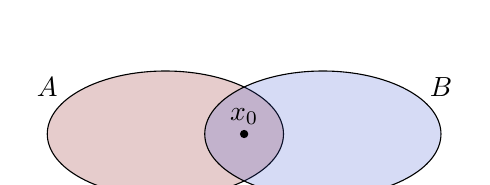
\begin{tikzpicture}
    \draw [fill=mred, fill opacity=0.2] (-1, 0) ellipse (1.5 and 0.8);
    \draw [fill=mblue, fill opacity=0.2] (1, 0) ellipse (1.5 and 0.8);
    \node [circ] {};
    \node [above] {$x_0$};
    \node at (-2.5, 0.6) {$A$};
    \node at (2.5, 0.6) {$B$};
  \end{tikzpicture}
\end{center}
Notice we have the following commutative diagram
\[
  \begin{tikzcd}[row sep=large]
    A \cap B \ar [r, hook] \ar[d, hook] & B\ar[d, hook] \\
    A \ar [r, hook] & X
  \end{tikzcd}
\]
where all arrows are the inclusion maps
(the hooks mean the maps are injective).
We can pick a basepoint $x_0 \in A \cap B$ for convenience.
We can consider what happens when we look at the fundamental groups
of each space.
\[
  \begin{tikzcd}[row sep=large]
    \pi_1(A \cap B, x_0) \ar[r] \ar[d] & \pi_1(B, x_0) \ar[d] \\
    \pi_1(A, x_0) \ar[r] & \pi_1(X, x_0)
  \end{tikzcd}
\]
where the arrows are the induced homomorphisms.
The Seifert-van Kampen theorem allows us to understand the group
$\pi_1(X, x_0)$ under the right conditions.

\begin{theorem}[Seifert-van Kampen theorem]
  Let $A$, $B$ be open subspaces of $X$ such that
  $X = A \cup B$, and $A$, $B$, $A \cap B$ are path-connected.
  Then for any $x_0 \in A \cap B$,
  we have
  \[
    \pi_1(X,x_0) = \pi_1(A,x_0) *_{\pi_1(A \cap B,x_0)} \pi_1(B,x_0).
  \]
\end{theorem}

\begin{example}
  Let $X = S^2$.
  We can cover $X$ with the open subsets $A = S^2 \setminus {N}$,
  $B = S^2 \setminus \set{S}$ for $N \neq S$ (for example the different
  north and south poles).
  Since $A$, $B$, $A \cap B$ are path-connected by the Seifert-van Kampen
  theorem we have that
  \[
    \pi_1(S^2,x_0) =
    \pi_1(A,x_0) *_{\pi_1(A \cap B,x_0)} \pi_1(B,x_0).
  \]
  However, since $A \cong B \cong \R^2$ we have that
  $\pi_1(A,x_0) \simeq \pi_1(B,x_0) \simeq 1$ and thus
  $\pi_1(S^2,x_0) = 1$.
\end{example}
\begin{remark}
  The proof in the example above works for any $S^2$ for any $n \geq 2$.
  However, it doesn't work when $n = 1$ because then $A \cap B$ is not
  path connected.
\end{remark}

\begin{example}
  \label{exmp:s-wedge-s}
  Let $X = S^1 \vee S^1$.
  We can cover $X$ by the open subsets $A$, $B$ as in the diagram
  \begin{center}
    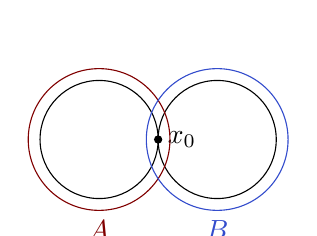
\begin{tikzpicture}[scale=0.75]
      \draw (-1, 0) circle [radius=1];
      \draw (1, 0) circle [radius=1];
      \node [circ] {};
      \node [right] {$x_0$};
      \draw [mred] (-1, 0) circle [radius=1.2];
      \draw [mblue] (1, 0) circle [radius=1.2];
      \node [below, mred] at (-1, -1.2) {$A$};
      \node [below, mblue] at (1, -1.2) {$B$};
    \end{tikzpicture}
  \end{center}
  such that each of $A$ and $B$ now look like this:
  \begin{center}
    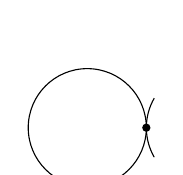
\begin{tikzpicture}[scale=0.75]
      \draw (0, 0) circle [radius=1];
      \draw (1, 0) arc (180:150:1); % intial deg:terminal deg:radius
      \draw (1, 0) arc (180:210:1);
      \node [circ] at (1, 0) {};
    \end{tikzpicture}
  \end{center}
  Notice that both of $A$, $B$ have a deformation retract to $S^1$.
  Since their intersection is contractible (and in particular path-connected)
  we get that
  \[
    \pi_1(X) =
    \pi_1(A) *_{\pi_1(A \cap B)} \pi_1(B) =
    \Z *_1 \Z =
    F_2.
  \]
\end{example}

We can now proceed to prove Seifert-van Kampen theorem.
\begin{proof}
  To be added
\end{proof}

\subsection{Applications of Seifert-van Kampen theorem}

\subsubsection{Presentation complexes}
\begin{theorem}
  Every group is the fundamental group of a polygonal complex.
\end{theorem}
\begin{proof}
  For simplicity we will only prove this for finitely presented groups.
  Let
  \[
    G := \langle s_1,\dots,s_n \mid r_1,\dots,r_m \rangle
  \]
  be a finitely presented group.
  In order to construct $G$ we choose a single point $*$ to be the
  $0$-skeleton and we connect it to $n$ unique $1$-cells $s_1,\dots,s_n$
  to obtain the $1$-skeleton $X^1$.
  Notice that since there is only one vertex these edges are connected to
  $*$ on both sides and form the shape of $S^1$.
  For each $1 \le i \le m$ we define a $2$-cell $\sigma_i$
  and paste its boundary to the edges that correspond to the word $r_i$.
  We denote this complex $X$.

  In order to calculate the fundamental group of $X$ we first
  use the Van-Kampen theorem to show inductively that
  \[
    \pi\del{\bigvee_{i=1}^{n} S^1_i} \cong F(s_1,\dots,s_n).
  \]
  Instead of showing this rigorously, we can see that
  the $1$-skeleton looks like
  \begin{center}
  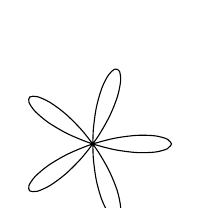
\begin{tikzpicture}
    \draw plot [smooth, samples=50, domain=0:180] (\x : {cos(5*\x)});
  \end{tikzpicture}
  \end{center}
  and just like in \Cref{exmp:s-wedge-s} see that the fundamental
  group is $F(s_1,\dots,s_n)$.

  Next by induction on $m$ we will show that
  $\pi_1(X,*) = \langle s_1,\dots,s_n \mid r_1,\dots,r_m \rangle$.
  We have shown the result for $m = 0$ above so we can assume that
  the hypothesis is true for $m - 1$ and prove it for $m$.
  Let $D_1 \subset D_2 \subset \sigma_m$ be two discs contained in $\sigma_m$.
  Define $A := X \setminus \overline{D_1}$ and $B := D_2$.
  We notice that there is a deformation retraction from $X^1$
  to $X^1 \cup \sigma_1 \cup \sigma_2 \cdot \cup \sigma_{m-1}$
  and thus from the induction hypothesis
  \[
    \pi_1(A) = \langle s_1,\dots,s_n \mid r_1,\dots,r_{m-1} \rangle.
  \]
  The space $B$ is contractible so $\pi_1(B) = 1$ and
  $A \cap B$ has a deformation retraction to $S^1$,
  which means that $\pi_1(A \cap B) = \pi_1(S^1) = \Z$.
  Let $c$ be the element that generates $\pi_1(A \cap B)$.
  Then $c$ is sent by the deformation retraction to the boundary
  of $\sigma_m$ (the word $r_m$ in $\pi_1(A)$).

  Using the Van-Kampen theorem we get that
  \begin{align*}
    \pi_1(X,*) &= \pi_1(A,*) *_{\pi_{A \cap B,*}} \pi_1(B,*) \\
               &= \langle s_1,\dots,s_n \mid r_1,\dots,r_{m-1} \rangle
                  *_{\langle c \mid \rangle} 1 \\
               &= \langle s_1,\dots,s_n \mid r_1,\dots,r_{m-1},r_m = 1 
               \rangle \\
               &= \langle s_1,\dots,s_n \mid r_1,\dots,r_m \rangle \\
               &= G
  \end{align*}
  which completes the proof
\end{proof}

\subsubsection{CW complexes}
\begin{theorem}
  \label{thm:two-skeleton-determines-fundamental-group}
  Let $X$ be a connected CW complex.
  Then $\pi_1(X) = \pi_1(X^{(2)})$.
\end{theorem}
\begin{proof}
  For simplicity we assume that $X$ contains a finite amount of
  cells of dimension greater than $2$.
  It suffices to show that if $X$ is a connected topological space
  and
  \[
    Y = X \cup D^n \setminus (\partial D^n \ni x \sim f(x) \in X)
  \]
  for $f \colon D^n \to X$ and $n > 2$ then $\pi_1(X) = \pi_2$.

  Indeed we can set $D_1 \subset D_2 \subset D^n$ and let
  $A := Y \setminus \overline{D_1}$ and $B := D_2$. We get that
  \[
    A \simeq_{\dfr} X \tand
    B \simeq_{\dfr} * \tand
    A \cap B \simeq_{\dfr} S^{n-1}
  \]
  and thus
  \[
    \pi_1(A) = \pi_1(X) \tand
    \pi_1(B) = 1 \tand
    \pi_1(A \cap B) = 1
  \]
  so from the Van-Kampen theorem
  \[
    \pi_1(Y) = \pi_1(X) *_{1} 1 = \pi_1(X)
  \]
  which completes the proof.
\end{proof}

\subsubsection{\texorpdfstring{$4$}{4}-dimensional manifolds}

\begin{lemma}
  \label{lem:three-dimensional-manifolds-csum}
  Let $M_1$ and $M_2$ be two topological
  manifolds of dimension $n \geq 3$.
  Then
  \[
    \pi_1(M_1 \# M_2) = \pi_1(M_1) * \pi_1(M_2).
  \]
\end{lemma}
\begin{proof}
  To be added.
  From an argument similar to the one seen in
  \Cref{thm:two-skeleton-determines-fundamental-group}
\end{proof}

\begin{theorem}
  Every finitely presented group is the fundamental group of a connected
  $4$-dimensional compact topological manifold.
\end{theorem}
\begin{proof}
  Let $G := \langle s_1,s_2,\dots,s_n \mid r_1,r_2,\dots,r_m \rangle$
  and let $X := \#^n (S^1 \times S^3)$.
  Notice that
  \[
    \pi_1(S^1 \times S^3) =
    \pi_1(S^1) \times \pi_1(S^3) =
    \Z \times 1 = \Z.
  \]
  We want to show inductively that
  \[
    \pi_1(X) =
    \pi_1(\#^n (S^1 \times S^3)) =
    \langle s_1,s_2,\dots,s_n \mid \rangle.
  \]
  For the base case let $n = 2$
  and let $A = B = S^1 \times S^3$.
  Since the $\dim A = \dim B = 4$ according to
  \Cref{lem:three-dimensional-manifolds-csum}
  we get that
  \[
    \pi_1(X) =
    \pi_1(A \# B) =
    \pi_1(A) * \pi_1(Z) =
    \Z * \Z =
    \langle s_1,s_2 \mid \rangle.
  \]
  For the step of the induction we can keep applying the lemma and get
  \begin{align*}
    \pi_1(\#^n (S_1 \times S^3)) &=
    \pi_1(\#^{n-1} (S_1 \times S^3)) * \pi_1(S_1 \times S^3) \\ &=
    \langle s_1,s_2,\dots,s_{n-1} \mid \rangle *_{1} \langle s_n \mid \rangle
                                                             \\ &=
    \langle s_1,s_2,\dots,s_{n} \mid \rangle
  \end{align*}
  where $s_i$ is represented by the $S^1$ factor of the $i$th summand of
  $\#^n (S^1 \times S^3)$.

  Each relation in $G$ can be represented by a loop in $X$.
  For example if $r_1 = s_1 s_2^{-1}$ then the loop would first
  go around the $S^1$ factor of the first summand, then
  around the $S^1$ factor of the second summand in reverse.
  We denote the loop corresponding to $r_i$ by $b_j$
  for all $1 \le i \le m$.

  Each loop $b_j$ has a tubular neighbourhood $N_j$, which
  is a copy of $S^1 \times D^3$ embedded in $X$.
  The boundaries of $N_j$ and $D^2 \times S^2$ are both homeomorphic to
  $S^1 \times S^2$ and thus we can cut out $N_j$ from $X$
  and paste a copy of $D^2 \times S^2$ in its place instead.
  For all $1 \le j \le m$ let $X_j$ be $X$ after this surgery for $b_j$.
  We can choose appropriate neighbourhoods $A$ and $B$ of
  $X \setminus \Int(N_j)$ and $D^2 \times S^2$ respectively so
  that $A \cap B \simeq_{\dfr} S^1 \times S^2$ and we can use
  the Van-Kampen theorem.
  Again from \Cref{lem:three-dimensional-manifolds-csum} we have
  \[
    \pi_1(X \setminus \Int(N_j)) = \langle s_1,s_2,\dots,s_n \mid \rangle
    \tand
    \pi_1(D^2 \times S^2) = 1
    \tand
    \pi_1(S^1 \times S^2) = \langle c \rangle,
  \]
  where $c = S^1 \times \set{*}$ for some $* \in S^2$.
  We see that $c$ is homotopic to $b_j$
  because $b_j = S^1 \times \set{*'} \subset N_j$
  and $c = S^1 \times \set{*} \subset S^1 \times S^2 = \partial N_j$
  which means that $c$ is just $b_j$ homotoped to the boundary
  of $N_j$.
  Therefore by the Van-Kampen theorem we get
  \[
    \pi_1(X_j) =
    \langle s_1,s_2,\dots,s_n \mid \rangle *_{\langle c \rangle} 1 =
    \langle s_1,s_2,\dots,s_n \mid r_j \rangle.
  \]
  Assuming we have done this process to $X$ for all $b_j$ 
  and denote the result $X'$ we get that
  \[
    \pi_1(X') =
    \langle s_1,s_2,\dots,s_n \mid r_1,r_2,\dots,r_m \rangle =
    G
  \]
  and since $X'$ is a connected $4$-dimensional
  compact topological manifold this completes the proof.
\end{proof}

\newpage

\section{Covering spaces and lifts}
\begin{remark}
  From now on, we assume all spaces are Hausdorff and path-connected.
\end{remark}

\begin{definition}[Covering]
  A surjective continuous map $p \colon \widetilde X \to X$ is called a
  covering of $X$ if for all $x \in X$ there exists an open neighbourhood
  $x \in U_x \subseteq X$ and a discrete space $D_x$ such that
  \[
    \pi^{-1}(U_x) = \bigsqcup_{d \in D_x} V_d
  \]
  and $\pi\vert_{V_d} \colon V_d \to U_x$ is a homeomorphism for every
  $d \in D_x$.
\end{definition}
\begin{definition}[Covering space]
  Under the conditions of the previous definition,
  the pair $(\widetilde X, p)$ is said to be a covering space of $X$.
\end{definition}
\begin{definition}[Sheet]
  Under the conditions of the previous definition,
  the sets $V_d$ are called sheets.
\end{definition}
\begin{remark}
  The sheets are uniquely determined by the homomorphism if $U_x$ is connected.
\end{remark}
\begin{remark}
  If $\widetilde X$ is path-connected we say that $p \colon \widetilde X \to X$
  is a path-connected covering.
\end{remark}

\noindent Some simple examples of covering maps are:
\begin{enumerate}
  \item[(1)] the identity map $\id \colon X \to X$;
  \item[(2)] the quotient map $p \colon \R \to \R / \Z = S^1$;
  \item[(3)] the map $p \colon S^1 \to S^1$ given by $p(z) = z^n$;
  \item[(4)] given covering maps $p_{\alpha} \colon \widetilde X_{\alpha} \to X$
    then the map $p =
    \bigsqcup p_{\alpha} \colon \bigsqcup_{\alpha} X_{\alpha} \to X$ is also
    a covering map;
  \item[(5)] given covering maps $p \colon \widetilde X \to X$ and
    $q \colon \widetilde Y \to Y$, then the map
    $p \times q \colon \widetilde X \times \widetilde Y \to X \times Y$
    is a covering map.
\end{enumerate}

\begin{example}
  We can expand on example $(2)$ by defining the covering maps more explicitly
  with $p(t) = \del{\cos(2 \pi t), \sin(2 \pi t)}$.
  We say that the base of the covering is $S^1$,
  and the covering space is $\R$.
  For any $x = (x_1,x_2) \in S^1$ we can consider (for example)
  the neighbourhood
  \[
    x \in U_x := \set{(x_1,x_2) \in S^1 \colon x_1 > 0}.
  \]
  We can see that the preimage of $U$ under $p$ is
  \[
    p^{-1}(U) = \bigsqcup_{n \in \Z} \del{n - \frac{1}{4}, n + \frac{1}{4}}
  \]
  and the sheets of the covering are $V_n = \del{n - 1/4, n + 1/4}$
  for $n \in \Z$.
\end{example}

% Picture examples

\begin{definition}[Lift]
  Let $p \colon \widetilde X \to X$ be a covering and
  let $f \colon Y \to X$ be continuous.
  A continuous map $\tilde f \colon Y \to \widetilde X$ is called a lift
  if it satisfies $f = p \circ \tilde f$.
\end{definition}

\begin{lemma}
  Let $\gamma \colon [0,1] \to X$ be a path.
  Then for all $x_0 \in p^{-1}(\gamma(0))$ there exists a unique lift
  $\tilde \gamma \colon [0,1] \to \widetilde X$ so that $\tilde \gamma(0) = x_0$.
\end{lemma}
\begin{proof}
  to be added.
\end{proof}

\begin{proposition}
  Let $X$ be path-connected,
  and let $p \colon \widetilde X \to X$ be a covering.
  Then for all $x,y \in X$ we have $\abs{p^{-1}(x)} = \abs{p^{-1}(y)}$.
\end{proposition}
\begin{proof}
  to be added.
\end{proof}

\begin{definition}[Degree of a covering]
  Let $X$ be path connected,
  let $x \in X$,
  and let $p \colon \widetilde X \to X$ be a covering.
  The constant $\abs{p^{-1}(x)}$ which is equal to the
  cardinality of $D_x$ is the same for all $x \in X$.
  This value is called the degree of the covering.
\end{definition}

\begin{proposition}
  Let $p \colon \widetilde X \to X$ be a covering,
  let $H \colon Y \times [0,1] \to X$ be a continuous map,
  and let $\tilde f \colon Y \times \set{0} \to \widetilde X$ be a lift
  of the map
  $f := H\vert_{Y \times \set{0}} \colon Y \times \set{0} \to X$.
  Then there exists a unique lift
  $\widetilde H \colon Y \times [0,1] \to \widetilde X$ of $H$ to $\widetilde X$
  such that $\widetilde H\vert_{Y \times \set{0}} = \tilde f$.
\end{proposition}
\begin{proof}
  to be added % (in the workshop).
\end{proof}

\begin{proposition}
  Let $p \colon (\widetilde X, \tilde{x_0}) \to (X, x_0)$ be a covering.
  Then
  \begin{enumerate}
    \item[(1)] The induced map
      $p_* \colon \pi_1(\widetilde X, \tilde{x_0}) \to \pi_1(X,x_0)$ is an
      injection.
    \item[(2)] Let $\gamma$ be a loop in $(X,x_0)$.
      Then $[\gamma] \in \widetilde G$ are the paths in $X$ if and only
      if the lift of $\gamma$ is a loop in $(\widetilde X, \tilde x_0)$.
    \item[(3)] Suppose that $X$, $\widetilde X$ are path-connected.
      Then there exists a bijection
      \[
        G / \widetilde G \longleftrightarrow p^{-1}(x_0)
      \]
      and in particular $\abs{p^{-1}(x_0)} = [G:H]$.
  \end{enumerate}
\end{proposition}
\begin{remark}
  We can denote $G := \pi_1(X,x_0)$ and
  also $\widetilde G = p_*(\pi_1(\widetilde X, \tilde{x_0}))$.
  Since $p_*$ is an injection we have that and from the proposition
  $\widetilde G \cong p_*(\pi_1(\widetilde X, \tilde{x_0}))$ is a subgroup
  of $G$.
\end{remark}
\begin{proof}
  to be added.
\end{proof}

\begin{definition}[Subgroup of a covering] % ???? what is the right name?
  The group $H = p_*(\pi_1(\widetilde X, \tilde{x_0})) \leqslant \pi_1(X,x_0)$
  is called the subgroup of $G$ given by the pointed space covering $p$.
\end{definition}

\begin{example}
  Let $p \colon \R \to S^1$ be the standard covering.
  In this case since $\R$ is contractible we have that
  $\pi_1(\R,0) = 1$ and for any equivalence class of loops
  $\gamma \in \pi_1(\R,0)$ we have that $p(\gamma)$ is the loops doing
  a net sum of zero circles on $S^1$ and thus $\widetilde G = 1$
  and indeed we have $G = G / \widetilde G \longleftrightarrow p^{-1}(x_0) = \Z$.
\end{example}

\begin{example}
  Let $p \colon S^1 \to S^1$ be given by $p(z) = z^n$.
  We then have that
  $\widetilde G = n\Z \leqslant \Z \simeq G$ and
  $p^{-1}(x_0) \longleftrightarrow \Z/n\Z$.
\end{example}

\begin{example}
  
\end{example}

\begin{example}
  Let $n \geq 2$.
  Then the covering $p \colon S^n \to \RP^n$ satisfies
  $\widetilde G = 1 \leqslant G$, and then
  \[
    |G| = \left[G:\widetilde G\right] = \abs{p^{-1}(x_0)} = 2
  \]
  which implies that $G$ is the cyclic group of order $2$.
\end{example}

\begin{example}
  We can see that
  \[
    \SO(3) =
    \set{A \in \Mat_n(\R) \colon A A^t = I \stand \det(A) = 1} \simeq
    \RP^3
  \]
  by considering the homeomorphism $D^3 \to \SO(3)$ defined by
  $v \mapsto A_v$ where $A_v$ is the matrix that rotates vectors
  by the angle $\pi \norm{v}$ around the axis spanned by $v$ (using
  the right hand rule) and $0 \mapsto I$.
\end{example}

\begin{theorem}[Unique lifting criterion]
  Let $p \colon (\widetilde X, \tilde x) \to (X, x)$ be a covering,
  let $f \colon (Y,y) \to (X,x)$ be a continuous map,
  and suppose that $Y$ is path connected and locally path connected.
  Then there exists a unique lift
  $\tilde f \colon (Y,y) \to (\widetilde X, \tilde x)$ if and only if
  $\im f_* \leqslant \im p_*$.
\end{theorem}
\begin{proof}
  to be added
\end{proof}

\newpage

\section{Theory of covering spaces}
\subsection{Automorphisms and subgroups}
\begin{definition}[Covering isomorphism]
  A map $f \colon \widetilde X \to \widetilde X'$ is called an isomorphism of
  coverings if it is a homeomorphism that satisfies $p = p' \circ f$.
  That is, it makes the following diagram commute.
  \begin{center}
  \begin{tikzcd}
\widetilde X \arrow[rd, "p"'] \arrow[rr, "f", dashed] &   & \widetilde X' \arrow[ld, "p'"] \\
                                                  & X &                           
  \end{tikzcd}
  \end{center}
  In this case, we say that the covering spaces $(\widetilde X, p)$,
  $(\widetilde X', p')$ are isomorphic.
\end{definition}

\begin{proposition}
  Let $X$, $\widetilde X$,
  and $\widetilde X'$ be connected and locally path-connected Hausdorff spaces,
  and let $p \colon (\widetilde X, \tilde x) \to (X, x)$ and
  $p' \colon (\widetilde X', \tilde x') \to (X, x)$ be their corresponding
  covering maps.
  Then there exists a unique covering isomorphism
  $f \colon (\widetilde X, \tilde x) \to (\widetilde X', \tilde x')$
  if and only if the subgroups given by the covering maps are equal,
  that is
  $\im p_* = \im p'_*$.
\end{proposition}
\begin{proof}
  to be added
\end{proof}

\begin{definition}[Covering automorphism]
  A covering isomorphism $f \colon \widetilde X \to \widetilde X$
  is called a covering automorphism (or a deck transformation).
  We can equivalently require that $f \colon \widetilde X \to \widetilde X$
  is a homeomorphism such that the following diagram
    \begin{center}
  \begin{tikzcd}
\widetilde X \arrow[rd, "p"'] \arrow[rr, "f", dashed] &   & \widetilde X \arrow[ld, "p"] \\
                                                  & X &                           
  \end{tikzcd}
  \end{center}
  commutes.
  We denote the automorphism group of the covering map
  $p \colon \widetilde X \to X$ by $\Aut(\widetilde X, p)$.
\end{definition}
\begin{remark}
  In some places this is denoted $\mathrm{Deck}(\widetilde X,p)$ or
  simply $\mathrm{Deck}(p)$ when the cover is clear from context.
\end{remark}

\begin{proposition}
  Let $p \colon (\widetilde X, \tilde x) \to (X, x)$ be a covering map between
  ``nice'' spaces.
  Denote $H = \im p_* \leqslant G = \pi_1(X,x)$.
  Then $\Aut(\widetilde X, p) \cong N_G(H) / H$.
\end{proposition}
\begin{proof}
  to be added
\end{proof}

\begin{definition}[Regular cover]
  A covering map $p \colon \widetilde X \to X$ so that
  $\widetilde X$ is connected and locally path connected
  is called a regular (or normal or Galois) if the standard
  group action given by $\Aut(\widetilde X, p)$ is transitive on some fiber
  $p^{-1}(x)$ (this implies that it is transitive on all fibers).
  That is, for all $\tilde x, \tilde y \in p^{-1}(x)$ there exists
  $f \in \Aut(\widetilde X, p)$ such that $f(\tilde x) = \tilde y$.
\end{definition}
\begin{remark}
  Recall that a group action is said to be free if for any two (possibly equal)
  elements of the set, there is at most one element of the group taking the
  first element to the second.
  Equivalently, an action is free if for all $g \in G$ and $x \in X$ then
  $g.x = x$ if and only if $g = 1$.
\end{remark}
\begin{remark}
  In general, a group action is called regular if it is both free and
  transitive.
  In this case, we have that $\Aut(\widetilde X, p)$ is always free so
  it is regular if and only if it is transitive.
  Moreover, an equivalent definition for a regular action is that
  for any two (possibly equal) elements of the set,
  there is a unique group element taking the first to the second.
\end{remark}

\begin{corollary}
  A covering map $p \colon \widetilde X \to X$ so that
  $\widetilde X$ is connected and locally path connected
  is regular if and only if its subgroup if normal, that is,
  $\im p_* \normalin \pi_1(X,x)$.
  In this case we have $\Aut(\widetilde X,p) = \pi_1(X) / \im p_*$.
\end{corollary}

\subsection{Covering space actions}
\begin{definition}[Covering space action]
  An action by homeomorphisms $G \actson Y$ such that for any point $y \in Y$
  there exists an open neighbourhood $y \in U \subset X$ so that
  $g.U \cap U = \emptyset$ for all $1 \neq g \in G$.
\end{definition}
\begin{remark}
  This type of group actions (which are not necessarily homeomorphisms)
  are also called \textit{properly discontinuous actions}.
\end{remark}

\begin{remark}
  We can notice that covering space actions are in particular free actions.
\end{remark}

\begin{remark}
  When considering the quotient space $G / Y$
  we mean the quotient space given by the equivalence
  relation generated by the orbits of the action
  ($y \sim gy$ for all $g \in G$).
  The topology of $G / Y$ is the quotient topology with that relation.
\end{remark}

\begin{remark}
  The quotient space $G / Y$ is not necessarily Hausdorff.
  For example, the action of $\Z \actson \R^2$ by
  $k.(x,y) = (2^k x, 2^{-k} y)$ is a covering space action,
  but the quotient is not Hausdorff.
\end{remark}

\begin{proposition}
  Let $p \colon \widetilde X \to X$ be a covering map,
  and let $X$ be path-connected and locally path connected.
  Then the action $\Aut(\widetilde X, p) \actson X$ is a covering space action.
\end{proposition}
\begin{proof}
  to be added.
\end{proof}

\begin{theorem}
  Let $G \actson \widetilde X$ be a covering space action.
  Then the quotient map $p \colon \widetilde X \to G / \widetilde X := X$
  is a regular covering map. % Check the := youre tired
\end{theorem}
\begin{proof}
  to be added.
\end{proof}

\begin{remark}
  Moreover, if $\widetilde X$ is path-connected and locally path-connected then
  we have $G = \Aut(\widetilde X, p)$.
\end{remark}

\subsection{The universal covering space}
\begin{definition}[Precisely $n$-connected space]
  A topological space $X$ is said to be precisely $n$-connected
  (or precisely $n$-simply connected) if every continuous map to $X$
  from $X$ to $S^n$ extends continuously to a map from $X$ to $D^{n+1}$.
\end{definition}

\begin{definition}[$n$-connected space]
  A topological space $X$ is said to be $n$-connected (or $n$-simply connected)
  if it is precisely $k$-connected for $-1 \le k \le n$.
  Equivalently, we have that a space is $n$-connected if its homotopy
  groups are trivial up to degree $n$.
\end{definition}
\begin{remark}
  General homotopy groups are hard to compute,
  and are discussed in the following algebraic topology course.
  For the purposes of this text it suffices to know that homotopy groups
  of degree $1$ are exactly the fundamental group.
\end{remark}

\begin{example}
  We have that
  \begin{enumerate}
    \item[(1)] any space is $(-2)$-connected;
    \item[(2)] a space is $(-1)$-connected precisely if it is nonempty;
    \item[(3)] a space is $0$-connected precisely if it is path-connected;
    \item[(4)] a space is $1$-connected precisely if it is simply connected. 
  \end{enumerate}
\end{example}

\begin{definition}[Universal covering space]
  A $1$-connected (nonempty, path-connected, simply connected)
  covering space is called a universal covering space.
\end{definition}

\begin{corollary}
  Let $p \colon \widetilde X \to X$ be a universal covering.
  Then,
  \begin{enumerate}
    \item[(1)] the universal covering is unique up to a covering isomorphism;
    \item[(2)] since $\widetilde X$ is simply connected we have
      $\im p_* \normalin \pi_1(X)$ and thus $\Aut(\widetilde X, p)$ is a
      transitive action on $p^{-1}(x)$;
    \item[(3)] $\Aut(\widetilde X, p) \cong \pi_1(X,x)$.
  \end{enumerate}
\end{corollary}

\subsection{Coverings and subgroups}
\begin{theorem}
  Let $p \colon \widetilde X \to X$ be the universal covering of $X$,
  let $X$ be path-connected and locally path connected,
  and let $H \leqslant G = \pi_1(X,x)$ be a subgroup.
  Then $G \actson \widetilde X$ TO BE ADDED.
\end{theorem}

\subsection{Conclusion}
\begin{remark}
  Let $p \colon (\widetilde X, \tilde x) \to (X, x)$ be the universal covering
  space.
  Denote $G = \pi_1(X,x)$.
  Then we have the following correspondence:
  \begin{center}
    \begin{tabular}{l|l}
  injection map  $\Aut(\widetilde X, p)$             & $G$                                \\
    connected pointed covers of $X$ & subgroups of $G$                   \\
    connected covers of $X$         & subgroups of $G$ up to conjugation \\
    covers of $X$                   & actions of $G$                    
    \end{tabular}
  \end{center}
\end{remark}

\newpage

\section{Universal covering space}
\subsection{Construction of the universal covering space}
\begin{definition}[slsc. space]
  A topological space $X$ is said to be
  semi locally simply connected (slsc.)
  if for any $x \in X$ there exists a path-connected neighbourhood
  $x \in U \subset X$ so that $i_*\del{(\pi_1(U,x))} = 1$ where
  $i \colon U \to X$ is the inclusion map.
  Equivalently, every loop in $U$ must be contractible, however,
  unlike local simply connectedness, we don't require the contraction
  to take place inside of $U$.
\end{definition}

\begin{example}
  Here are some examples and nonexamples of slsc. spaces:
  \begin{enumerate}
    \item[(1)] topological manifolds are slsc spaces;
    \item[(2)] CW complexes are slsc spaces;
    \item[(3)] the Hawaiian earring which is defined as
      \[
        X = \bigcup_{n=1}^{\infty} S^1\del{\frac{1}{n}, \frac{1}{n}}
      \]
      is not a slsc space;
    \item[(4)] the cone
      \[
        Y = C(X) = X \times [0,1] / X \times \set{0}
      \]
      is a slsc space.
  \end{enumerate}
\end{example}

\begin{theorem}
  Let $X$ be connected, locally path-connected, and slsc.
  Then $X$ has a universal covering.
\end{theorem}
\begin{proof}
  to be added
\end{proof}

\begin{lemma}
  Let $X$, $Y$, $Z$ be path-connected, locally path-connnected,
  and semi locally simply connected,
  let $p$, $q$, $r$ be surjective maps such that the following diagram
  commutes.
  \begin{center}
  \begin{tikzcd}
                   & Z \arrow[rd, "p"] \arrow[ld, "q"'] &   \\
  Y \arrow[rr, "r"'] &                                    & X
  \end{tikzcd}
  \end{center}
  Then if two of the three maps are covering maps, then so is the third.
\end{lemma}
\begin{proof}
  to be added
\end{proof}

\subsection{Cayley graphs and Cayley complexes}
\subsection{Schreier graphes and Schreier complexes}



% \begin{exa}



% Any group has a representation

% Add example of pasting all sides of the triangle to one another.

% Finitely generated groups

% locally homeomorphic to R but not hausdorff

% All groups are quotient of free groups


\end{document}
